\chapter{含参量积分}

\section{含参量正常积分}

从本章开始我们讨论多元函数的各种积分问题,首先研究含参量积分. 设 \(f\left( {x,y}\right)\) 是定义在矩形区域 \(R = \left\lbrack  {a,b}\right\rbrack   \times  \left\lbrack  {c,d}\right\rbrack\) 上的二元函数\footnote{在建立含参量积分的概念和讨论其连续性与可微性时,矩形区域 \(\left\lbrack  {a,b}\right\rbrack   \times  \left\lbrack  {c,d}\right\rbrack\) 可改为更一般的区域 \(I \times  \left\lbrack  {c,d}\right\rbrack\) ,其中 \(I\) 为区间.}. 当 \(x\) 取 \(\left\lbrack  {a,b}\right\rbrack\) 上某定值时,函数 \(f\left( {x,y}\right)\) 则是定义在 \(\left\lbrack  {c,d}\right\rbrack\) 上以 \(y\) 为自变量的一元函数. 倘若这时 \(f\left( {x,y}\right)\) 在 \(\left\lbrack  {c,d}\right\rbrack\) 上可积,则其积分值是 \(x\) 在 \(\left\lbrack  {a,b}\right\rbrack\) 上取值的函数,记它为 \(\varphi \left( x\right)\) ,就有
\[
\varphi \left( x\right)  = {\int }_{c}^{d}f\left( {x,y}\right) \mathrm{d}y,x \in  \left\lbrack  {a,b}\right\rbrack  . \tag{1}
\]
一般地,设 \(f\left( {x,y}\right)\) 为定义在区域 \(G = \{ \left( {x,y}\right)  \mid\)  \(c\left( x\right)  \leq  y \leq  d\left( x\right) ,a \leq  x \leq  b\}\) 上的二元函数,其中 \(c\left( x\right) ,d\left( x\right)\) 为定义在 \(\left\lbrack  {a,b}\right\rbrack\) 上的连续函数 (图 19-1),若对于 \(\left\lbrack  {a,b}\right\rbrack\) 上每一固定的 \(x\) 值, \(f\left( {x,y}\right)\) 作为 \(y\) 的函数在闭区间 \(\left\lbrack  {c\left( x\right) ,d\left( x\right) }\right\rbrack\) 上可积,则其积分值是 \(x\) 在 \(\left\lbrack  {a,b}\right\rbrack\) 上取值的函数,记作 \(F\left( x\right)\) 时, 就有
\[
F\left( x\right)  = {\int }_{c\left( x\right) }^{d\left( x\right) }f\left( {x,y}\right) \mathrm{d}y,x \in  \left\lbrack  {a,b}\right\rbrack  . \tag{2}
\]
\begin{figure}
	\centering
	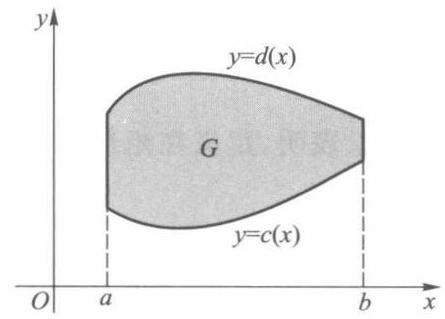
\includegraphics[width=.3\textwidth]{images/P147.jpg}
	\caption{图 $19-1$}
	\label{fig:P147}
\end{figure}

用积分形式所定义的这两个函数 (1) 与 (2),通称为定义在 \(\left\lbrack  {a,b}\right\rbrack\) 上含参量 \(x\) 的 (正常) 积分, 或简称含参量积分.

下面讨论含参量积分的连续性、可微性与可积性.

%定理 19.1
\begin{theorem}{}{the:}

\end{theorem}
 (连续性) 若二元函数 \(f\left( {x,y}\right)\) 在矩形区域 \(R = \left\lbrack  {a,b}\right\rbrack   \times  \left\lbrack  {c,d}\right\rbrack\) 上连续,则函数
\[
\varphi \left( x\right)  = {\int }_{c}^{d}f\left( {x,y}\right) \mathrm{d}y
\]
在 \(\left\lbrack  {a,b}\right\rbrack\) 上连续.

%证
\begin{proof}

\end{proof}
设 \(x \in  \left\lbrack  {a,b}\right\rbrack\) ,对充分小的 \({\Delta x}\) ,有 \(x + {\Delta x} \in  \left\lbrack  {a,b}\right\rbrack\) (若 \(x\) 为区间的端点,则仅考虑 \({\Delta x} > 0\) 或 \({\Delta x} < 0)\) ,于是
\[
\varphi \left( {x + {\Delta x}}\right)  - \varphi \left( x\right)  = {\int }_{c}^{d}\left\lbrack  {f\left( {x + {\Delta x},y}\right)  - f\left( {x,y}\right) }\right\rbrack  \mathrm{d}y. \tag{3}
\]
由于 \(f\left( {x,y}\right)\) 在有界闭域 \(R\) 上连续,从而一致连续,即对任给的正数 \(\varepsilon\) ,总存在某个正数 \(\delta\) ,对 \(R\) 内任意两点 \(\left( {{x}_{1},{y}_{1}}\right)\) 与 \(\left( {{x}_{2},{y}_{2}}\right)\) ,只要
\[
\left| {{x}_{1} - {x}_{2}}\right|  < \delta ,\left| {{y}_{1} - {y}_{2}}\right|  < \delta ,
\]
就有
\[
\left| {f\left( {{x}_{1},{y}_{1}}\right)  - f\left( {{x}_{2},{y}_{2}}\right) }\right|  < \varepsilon . \tag{4}
\]
所以由 (3),(4) 可推得: 当 \(\left| {\Delta x}\right|  < \delta\) 时,
\[
\left| {\varphi \left( {x + {\Delta x}}\right)  - \varphi \left( x\right) }\right|  \leq  {\int }_{c}^{d}\left| {f\left( {x + {\Delta x},y}\right)  - f\left( {x,y}\right) }\right| \mathrm{d}y
\]
\[
< {\int }_{c}^{d}\varepsilon \mathrm{d}x = \varepsilon \left( {d - c}\right) .
\]
这就证明了 \(\varphi \left( x\right)\) 在 \(\left\lbrack  {a,b}\right\rbrack\) 上连续.

同理可证: 若 \(f\left( {x,y}\right)\) 在矩形区域 \(R\) 上连续,则含参量 \(y\) 的积分
\[
\psi \left( y\right)  = {\int }_{a}^{b}f\left( {x,y}\right) \mathrm{d}x \tag{5}
\]
在 \(\left\lbrack  {c,d}\right\rbrack\) 上连续.

对于定理 19.1 的结论也可以写成如下的形式: 若 \(f\left( {x,y}\right)\) 在矩形区域 \(R\) 上连续,则对任何 \({x}_{0} \in  \left\lbrack  {a,b}\right\rbrack\) ,都有
\[
\mathop{\lim }\limits_{{x \rightarrow  {x}_{0}}}{\int }_{c}^{d}f\left( {x,y}\right) \mathrm{d}y = {\int }_{c}^{d}\mathop{\lim }\limits_{{x \rightarrow  {x}_{0}}}f\left( {x,y}\right) \mathrm{d}y.
\]
这个结论表明, 定义在矩形区域上的连续函数, 其极限运算与积分运算的顺序是可以交换的.

%定理 19.2
\begin{theorem}{}{the:}

\end{theorem}
 (连续性) 设二元函数 \(f\left( {x,y}\right)\) 在区域
\[
G = \{ \left( {x,y}\right)  \mid  c\left( x\right)  \leq  y \leq  d\left( x\right) ,a \leq  x \leq  b\}
\]
上连续,其中 \(c\left( x\right) ,d\left( x\right)\) 为 \(\left\lbrack  {a,b}\right\rbrack\) 上的连续函数,则函数
\[
F\left( x\right)  = {\int }_{c\left( x\right) }^{d\left( x\right) }f\left( {x,y}\right) \mathrm{d}y \tag{6}
\]
在 \(\left\lbrack  {a,b}\right\rbrack\) 上连续.

%证
\begin{proof}

\end{proof}
对积分 (6) 用换元积分法, 令
\[
y = c\left( x\right)  + t\left( {d\left( x\right)  - c\left( x\right) }\right) .
\]
当 \(y\) 在 \(c\left( x\right)\) 与 \(d\left( x\right)\) 之间取值时, \(t\) 在 \(\left\lbrack  {0,1}\right\rbrack\) 上取值,且
\[
\mathrm{d}y = \left( {d\left( x\right)  - c\left( x\right) }\right) \mathrm{d}t.
\]
所以从 (6) 式可得
\[
F\left( x\right)  = {\int }_{c\left( x\right) }^{d\left( x\right) }f\left( {x,y}\right) \mathrm{d}y
\]
\[
= {\int }_{0}^{1}f\left( {x,c\left( x\right)  + t\left( {d\left( x\right)  - c\left( x\right) }\right) }\right) \left( {d\left( x\right)  - c\left( x\right) }\right) \mathrm{d}t.
\]
由于被积函数
\[
f\left( {x,c\left( x\right)  + t\left( {d\left( x\right)  - c\left( x\right) }\right) }\right) \left( {d\left( x\right)  - c\left( x\right) }\right)
\]
在矩形区域 \(\left\lbrack  {a,b}\right\rbrack   \times  \left\lbrack  {0,1}\right\rbrack\) 上连续,由定理 19.1 得积分 (6) 所确定的函数 \(F\left( x\right)\) 在 \(\left\lbrack  {a,b}\right\rbrack\) 上连续.

下面讨论含参量积分的求导运算与积分运算的可交换性.

%定理 19.3
\begin{theorem}{}{the:}

\end{theorem}
 (可微性) 若函数 \(f\left( {x,y}\right)\) 与其偏导数 \(\frac{\partial }{\partial x}f\left( {x,y}\right)\) 都在矩形区域 \(R =\)  \(\left\lbrack  {a,b}\right\rbrack   \times  \left\lbrack  {c,d}\right\rbrack\) 上连续,则
\[
\varphi \left( x\right)  = {\int }_{c}^{d}f\left( {x,y}\right) \mathrm{d}y
\]
在 \(\left\lbrack  {a,b}\right\rbrack\) 上可微,且
\[
\frac{\mathrm{d}}{\mathrm{d}x}{\int }_{c}^{d}f\left( {x,y}\right) \mathrm{d}y = {\int }_{c}^{d}\frac{\partial }{\partial x}f\left( {x,y}\right) \mathrm{d}y.
\]
%证
\begin{proof}

\end{proof}
对于 \(\left\lbrack  {a,b}\right\rbrack\) 内任一点 \(x\) ,设 \(x + {\Delta x} \in  \left\lbrack  {a,b}\right\rbrack\) (若 \(x\) 为区间端点,则讨论单侧导数), 则
\[
\frac{\varphi \left( {x + {\Delta x}}\right)  - \varphi \left( x\right) }{\Delta x} = {\int }_{c}^{d}\frac{f\left( {x + {\Delta x},y}\right)  - f\left( {x,y}\right) }{\Delta x}\mathrm{\;d}y.
\]
由微分学的拉格朗日中值定理及 \({f}_{x}\left( {x,y}\right)\) 在有界闭域 \(R\) 上连续 (从而一致连续),对任给正数 \(\varepsilon\) ,存在正数 \(\delta\) ,只要当 \(\left| {\Delta x}\right|  < \delta\) 时,就有
\[
\left| {\frac{f\left( {x + {\Delta x},y}\right)  - f\left( {x,y}\right) }{\Delta x} - {f}_{x}\left( {x,y}\right) }\right|
\]
\[
= \left| {{f}_{x}\left( {x + {\theta \Delta x},y}\right)  - {f}_{x}\left( {x,y}\right) }\right|  < \varepsilon ,
\]
其中 \(\theta  \in  \left( {0,1}\right)\) . 因此
\[
\left| {\frac{\Delta \varphi }{\Delta x} - {\int }_{c}^{d}{f}_{x}\left( {x,y}\right) \mathrm{d}y}\right|
\]
\[
\leq  {\int }_{c}^{d}\left| {\frac{f\left( {x + {\Delta x},y}\right)  - f\left( {x,y}\right) }{\Delta x} - {f}_{x}\left( {x,y}\right) }\right| \mathrm{d}y
\]
\[
< \varepsilon \left( {d - c}\right) \text{ . }
\]
这就证得对一切 \(x \in  \left\lbrack  {a,b}\right\rbrack\) ,有
\[
\frac{\mathrm{d}}{\mathrm{d}x}\varphi \left( x\right)  = {\int }_{c}^{d}\frac{\partial }{\partial x}f\left( {x,y}\right) \mathrm{d}y.
\]
%定理 19.4
\begin{theorem}{}{the:}

\end{theorem}
 (可微性) 设 \(f\left( {x,y}\right) ,{f}_{x}\left( {x,y}\right)\) 在 \(R = \left\lbrack  {a,b}\right\rbrack   \times  \left\lbrack  {p,q}\right\rbrack\) 上连续, \(c\left( x\right) ,d\left( x\right)\) 为定义在 \(\left\lbrack  {a,b}\right\rbrack\) 上其值含于 \(\left\lbrack  {p,q}\right\rbrack\) 内的可微函数,则函数
\[
F\left( x\right)  = {\int }_{c\left( x\right) }^{d\left( x\right) }f\left( {x,y}\right) \mathrm{d}y
\]
在 \(\left\lbrack  {a,b}\right\rbrack\) 上可微,且
\[
{F}^{\prime }\left( x\right)  = {\int }_{c\left( x\right) }^{d\left( x\right) }{f}_{x}\left( {x,y}\right) \mathrm{d}y + f\left( {x,d\left( x\right) }\right) {d}^{\prime }\left( x\right)  - f\left( {x,c\left( x\right) }\right) {c}^{\prime }\left( x\right) . \tag{7}
\]
%证
\begin{proof}

\end{proof}
把 \(F\left( x\right)\) 看作复合函数
\[
F\left( x\right)  = H\left( {x,c,d}\right)  = {\int }_{c}^{d}f\left( {x,y}\right) \mathrm{d}y,
\]
\[
c = c\left( x\right) ,d = d\left( x\right) .
\]
由复合函数求导法则及变限积分的求导法则, 有
\[
\frac{\mathrm{d}}{\mathrm{d}x}F\left( x\right)  = \frac{\partial H}{\partial x} + \frac{\partial H}{\partial c}\frac{\mathrm{d}c}{\mathrm{\;d}x} + \frac{\partial H}{\partial d}\frac{\mathrm{d}d}{\mathrm{\;d}x}
\]
\[
= {\int }_{c\left( x\right) }^{d\left( x\right) }{f}_{x}\left( {x,y}\right) \mathrm{d}y + f\left( {x,d\left( x\right) }\right) {d}^{\prime }\left( x\right)  - f\left( {x,c\left( x\right) }\right) {c}^{\prime }\left( x\right) .
\]
关于函数 \(\varphi \left( x\right)\) 和 \(F\left( x\right)\) 的可积性,可由定理 19.1 与定理 19.2 推得.

%定理 19.5
\begin{theorem}{}{the:}

\end{theorem}
 (可积性) 若 \(f\left( {x,y}\right)\) 在矩形区域 \(R = \left\lbrack  {a,b}\right\rbrack   \times  \left\lbrack  {c,d}\right\rbrack\) 上连续,则 \(\varphi \left( x\right)\) 和 \(\psi \left( y\right)\) 分别在 \(\left\lbrack  {a,b}\right\rbrack\) 和 \(\left\lbrack  {c,d}\right\rbrack\) 上可积.

这就是说: 在 \(f\left( {x,y}\right)\) 连续性假设下,同时存在两个求积顺序不同的积分:
\[
{\int }_{a}^{b}\left\lbrack  {{\int }_{c}^{d}f\left( {x,y}\right) \mathrm{d}y}\right\rbrack  \mathrm{d}x\text{ 与 }{\int }_{c}^{d}\left\lbrack  {{\int }_{a}^{b}f\left( {x,y}\right) \mathrm{d}x}\right\rbrack  \mathrm{d}y.
\]
为书写简便起见, 今后将上述两个积分写作
\[
{\int }_{a}^{b}\mathrm{\;d}x{\int }_{c}^{d}f\left( {x,y}\right) \mathrm{d}y\text{ 与 }{\int }_{c}^{d}\mathrm{\;d}y{\int }_{a}^{b}f\left( {x,y}\right) \mathrm{d}x,
\]
前者表示 \(f\left( {x,y}\right)\) 先对 \(y\) 求积然后对 \(x\) 求积,后者则求积顺序相反. 它们统称为累次积分, 或更确切地称为二次积分. 下面的定理指出,在 \(f\left( {x,y}\right)\) 连续性假设下,累次积分与求积顺序无关.

%定理 19.6
\begin{theorem}{}{the:}

\end{theorem}
 若 \(f\left( {x,y}\right)\) 在矩形区域 \(R = \left\lbrack  {a,b}\right\rbrack   \times  \left\lbrack  {c,d}\right\rbrack\) 上连续,则
\[
{\int }_{a}^{b}\mathrm{\;d}x{\int }_{c}^{d}f\left( {x,y}\right) \mathrm{d}y = {\int }_{c}^{d}\mathrm{\;d}y{\int }_{a}^{b}f\left( {x,y}\right) \mathrm{d}x. \tag{8}
\]
%证
\begin{proof}

\end{proof}
记
\[
{\varphi }_{1}\left( u\right)  = {\int }_{a}^{u}\mathrm{\;d}x{\int }_{c}^{d}f\left( {x,y}\right) \mathrm{d}y,
\]
\[
{\varphi }_{2}\left( u\right)  = {\int }_{c}^{d}\mathrm{\;d}y{\int }_{a}^{u}f\left( {x,y}\right) \mathrm{d}x,
\]
其中 \(u \in  \left\lbrack  {a,b}\right\rbrack\) ,现在分别求 \({\varphi }_{1}\left( u\right)\) 与 \({\varphi }_{2}\left( u\right)\) 的导数.
\[
{\varphi }_{1}^{\prime }\left( u\right)  = \frac{\mathrm{d}}{\mathrm{d}u}{\int }_{a}^{u}\varphi \left( x\right) \mathrm{d}x = \varphi \left( u\right) .
\]
对于 \({\varphi }_{2}\left( u\right)\) ,令 \(H\left( {u,y}\right)  = {\int }_{a}^{u}f\left( {x,y}\right) \mathrm{d}x\) ,则有
\[
{\varphi }_{2}\left( u\right)  = {\int }_{c}^{d}H\left( {u,y}\right) \mathrm{d}y.
\]
因为 \(H\left( {u,y}\right)\) 与 \({H}_{u}\left( {u,y}\right)  = f\left( {u,y}\right)\) 都在 \(R\) 上连续,由定理 19.3,
\[
{\varphi }_{2}^{\prime }\left( u\right)  = \frac{\mathrm{d}}{\mathrm{d}u}{\int }_{c}^{d}H\left( {u,y}\right) \mathrm{d}y = {\int }_{c}^{d}{H}_{u}\left( {u,y}\right) \mathrm{d}y
\]
\[
= {\int }_{c}^{d}f\left( {u,y}\right) \mathrm{d}y = \varphi \left( u\right) .
\]
故得 \({\varphi }_{1}^{\prime }\left( u\right)  = {\varphi }_{2}^{\prime }\left( u\right)\) ,因此对一切 \(u \in  \left\lbrack  {a,b}\right\rbrack\) ,有
\[
{\varphi }_{1}\left( u\right)  = {\varphi }_{2}\left( u\right)  + k\;\left( {k\text{ 为常数 }}\right) .
\]
当 \(u = a\) 时, \({\varphi }_{1}\left( a\right)  = {\varphi }_{2}\left( a\right)  = 0\) ,于是 \(k = 0\) ,即得
\[
{\varphi }_{1}\left( u\right)  = {\varphi }_{2}\left( u\right) ,u \in  \left\lbrack  {a,b}\right\rbrack  .
\]
取 \(u = b\) ,就得到所要证明的 (8) 式.

%例 1
\begin{example}

\end{example}
求 \(\mathop{\lim }\limits_{{\alpha  \rightarrow  0}}{\int }_{\alpha }^{1 + \alpha }\frac{\mathrm{d}x}{1 + {x}^{2} + {\alpha }^{2}}\) .

%解
\begin{solution}

\end{solution}
记 \(I\left( \alpha \right)  = {\int }_{\alpha }^{1 + \alpha }\frac{\mathrm{d}x}{1 + {x}^{2} + {\alpha }^{2}}\) . 由于 \(\alpha ,1 + \alpha ,\frac{1}{1 + {x}^{2} + {\alpha }^{2}}\) 都是 \(\alpha\) 和 \(x\) 的连续函数,由定理 19.2 知 \(I\left( \alpha \right)\) 在 \(\alpha  = 0\) 处连续,所以
\[
\mathop{\lim }\limits_{{\alpha  \rightarrow  0}}I\left( \alpha \right)  = I\left( 0\right)  = {\int }_{0}^{1}\frac{\mathrm{d}x}{1 + {x}^{2}} = \frac{\pi }{4}.
\]
%例 2
\begin{example}

\end{example}
设 \(f\left( x\right)\) 在 \(x = 0\) 的某个邻域 \(U\) 上连续,验证当 \(x \in  U\) 时,函数
\[
\varphi \left( x\right)  = \frac{1}{\left( {n - 1}\right) !}{\int }_{0}^{x}{\left( x - t\right) }^{n - 1}f\left( t\right) \mathrm{d}t \tag{9}
\]
的 \(n\) 阶导数存在,且 \({\varphi }^{\left( n\right) }\left( x\right)  = f\left( x\right)\) .

%解
\begin{solution}

\end{solution}
由于 (9) 中被积函数 \(F\left( {x,t}\right)  = {\left( x - t\right) }^{n - 1}f\left( t\right)\) 及其偏导数 \({F}_{x}\left( {x,t}\right)\) 在 \(U \times  U\) 上连续, 于是由定理 19.4 可得
\[
{\varphi }^{\prime }\left( x\right)  = \frac{1}{\left( {n - 1}\right) !}{\int }_{0}^{x}\left( {n - 1}\right) {\left( x - t\right) }^{n - 2}f\left( t\right) \mathrm{d}t + \frac{1}{\left( {n - 1}\right) !}{\left( x - x\right) }^{n - 1}f\left( x\right)
\]
\[
= \frac{1}{\left( {n - 2}\right) !}{\int }_{0}^{x}{\left( x - t\right) }^{n - 2}f\left( t\right) \mathrm{d}t.
\]
同理
\[
{\varphi }^{\prime \prime }\left( x\right)  = \frac{1}{\left( {n - 3}\right) !}{\int }_{0}^{x}{\left( x - t\right) }^{n - 3}f\left( t\right) \mathrm{d}t.
\]
如此继续下去,求得 \(k\) 阶导数为
\[
{\varphi }^{\left( k\right) }\left( x\right)  = \frac{1}{\left( {n - k - 1}\right) !}{\int }_{0}^{x}{\left( x - t\right) }^{n - k - 1}f\left( t\right) \mathrm{d}t,\;k = 1,2,\cdots ,n - 1.
\]
特别当 \(k = n - 1\) 时有
\[
{\varphi }^{\left( n - 1\right) }\left( x\right)  = {\int }_{0}^{x}f\left( t\right) \mathrm{d}t,
\]
于是 \({\varphi }^{\left( n\right) }\left( x\right)  = f\left( x\right)\) . 附带说明,当 \(x = 0\) 时, \(\varphi \left( x\right)\) 及其各阶导数为
\[
\varphi \left( 0\right)  = {\varphi }^{\prime }\left( 0\right)  = \cdots  = {\varphi }^{\left( n - 1\right) }\left( 0\right)  = 0.
\]
%例 3
\begin{example}

\end{example}
求 \(I = {\int }_{0}^{1}\frac{{x}^{b} - {x}^{a}}{\ln x}\mathrm{\;d}x\;\left( {b > a > 0}\right)\) .

%解
\begin{solution}

\end{solution}
因为 \({\int }_{a}^{b}{x}^{y}\mathrm{\;d}y = \frac{{x}^{b} - {x}^{a}}{\ln x}\) ,所以
\[
I = {\int }_{0}^{1}\mathrm{\;d}x{\int }_{a}^{b}{x}^{y}\mathrm{\;d}y.
\]
由于函数 \({x}^{y}\) 在 \(R = \left\lbrack  {0,1}\right\rbrack   \times  \left\lbrack  {a,b}\right\rbrack\) 上满足定理 19.6 的条件,所以交换积分顺序得到
\[
I = {\int }_{a}^{b}\mathrm{\;d}y{\int }_{0}^{1}{x}^{y}\mathrm{\;d}x = {\int }_{a}^{b}\frac{1}{1 + y}\mathrm{\;d}y = \ln \frac{1 + b}{1 + a}.
\]
%例 4
\begin{example}

\end{example}
计算积分
\[
I = {\int }_{0}^{1}\frac{\ln \left( {1 + x}\right) }{1 + {x}^{2}}\mathrm{\;d}x.
\]
%解
\begin{solution}

\end{solution}
考虑含参量积分
\[
\varphi \left( \alpha \right)  = {\int }_{0}^{1}\frac{\ln \left( {1 + {\alpha x}}\right) }{1 + {x}^{2}}\mathrm{\;d}x,\;\alpha  \in  \left\lbrack  {0,1}\right\rbrack  .
\]
显然 \(\varphi \left( 0\right)  = 0,\varphi \left( 1\right)  = I\) ,且函数 \(\frac{\ln \left( {1 + {\alpha x}}\right) }{1 + {x}^{2}}\) 在 \(R = \left\lbrack  {0,1}\right\rbrack   \times  \left\lbrack  {0,1}\right\rbrack\) 上满足定理 19.3 的条件, 于是
\[
{\varphi }^{\prime }\left( \alpha \right)  = {\int }_{0}^{1}\frac{x}{\left( {1 + {x}^{2}}\right) \left( {1 + {\alpha x}}\right) }\mathrm{d}x.
\]
因为
\[
\frac{x}{\left( {1 + {x}^{2}}\right) \left( {1 + {\alpha x}}\right) } = \frac{1}{1 + {\alpha }^{2}}\left( {\frac{\alpha  + x}{1 + {x}^{2}} - \frac{\alpha }{1 + {\alpha x}}}\right) ,
\]
所以
\[
{\varphi }^{\prime }\left( \alpha \right)  = \frac{1}{1 + {\alpha }^{2}}\left( {{\int }_{0}^{1}\frac{\alpha }{1 + {x}^{2}}\mathrm{\;d}x + {\int }_{0}^{1}\frac{x}{1 + {x}^{2}}\mathrm{\;d}x - {\int }_{0}^{1}\frac{\alpha }{1 + {\alpha x}}\mathrm{\;d}x}\right)
\]
\[
= \frac{1}{1 + {\alpha }^{2}}\left\lbrack  {{\left. \alpha \arctan x\right| }_{0}^{1} + {\left. \frac{1}{2}\ln \left( 1 + {x}^{2}\right) \right| }_{0}^{1} - {\left. \ln \left( 1 + \alpha x\right) \right| }_{0}^{1}}\right\rbrack
\]
\[
= \frac{1}{1 + {\alpha }^{2}}\left\lbrack  {\alpha  \cdot  \frac{\pi }{4} + \frac{1}{2}\ln 2 - \ln \left( {1 + \alpha }\right) }\right\rbrack  .
\]
因此
\[
{\int }_{0}^{1}{\varphi }^{\prime }\left( \alpha \right) \mathrm{d}\alpha  = {\int }_{0}^{1}\frac{1}{1 + {\alpha }^{2}}\left\lbrack  {\frac{\pi }{4}\alpha  + \frac{1}{2}\ln 2 - \ln \left( {1 + \alpha }\right) }\right\rbrack  \mathrm{d}\alpha
\]
\[
= {\left. \frac{\pi }{8}\ln \left( 1 + {\alpha }^{2}\right) \right| }_{0}^{1} + {\left. \frac{1}{2}\ln 2\arctan \alpha \right| }_{0}^{1} - \varphi \left( 1\right)
\]
\[
= \frac{\pi }{8}\ln 2 + \frac{\pi }{8}\ln 2 - \varphi \left( 1\right)
\]
\[
= \frac{\pi }{4}\ln 2 - \varphi \left( 1\right) \text{ . }
\]
另一方面,
\[
{\int }_{0}^{1}{\varphi }^{\prime }\left( \alpha \right) \mathrm{d}\alpha  = \varphi \left( 1\right)  - \varphi \left( 0\right)  = \varphi \left( 1\right) ,
\]
所以 \(I = \varphi \left( 1\right)  = \frac{\pi }{8}\ln 2\) .

\subsection{习题 19.1}

1. 设 \(f\left( {x,y}\right)  = \operatorname{sgn}\left( {x - y}\right)\) (这个函数在 \(x = y\) 时不连续),试证由含参量积分
\[
F\left( y\right)  = {\int }_{0}^{1}f\left( {x,y}\right) \mathrm{d}x
\]
所确定的函数在 \(\left( {-\infty , + \infty }\right)\) 上连续,并作函数 \(F\left( y\right)\) 的图像.

2. 求下列极限:

(1) \(\mathop{\lim }\limits_{{\alpha  \rightarrow  0}}{\int }_{-1}^{1}\sqrt{{x}^{2} + {\alpha }^{2}}\mathrm{\;d}x\) ;

(2) \(\mathop{\lim }\limits_{{\alpha  \rightarrow  0}}{\int }_{0}^{2}{x}^{2}\cos {\alpha x}\mathrm{\;d}x\) .

3. 设 \(F\left( x\right)  = {\int }_{x}^{{x}^{2}}{\mathrm{e}}^{-x{y}^{2}}\mathrm{\;d}y\) ,求 \({F}^{\prime }\left( x\right)\) .

4. 应用对参量的微分法,求下列积分:

(1) \({\int }_{0}^{\frac{\pi }{2}}\ln \left( {{a}^{2}{\sin }^{2}x + {b}^{2}{\cos }^{2}x}\right) \mathrm{d}x\left( {{a}^{2} + {b}^{2} \neq  0}\right)\) ;

(2) \({\int }_{0}^{\pi }\ln \left( {1 - {2a}\cos x + {a}^{2}}\right) \mathrm{d}x\) .

5. 应用积分号下的积分法, 求下列积分:

(1) \({\int }_{0}^{1}\sin \left( {\ln \frac{1}{x}}\right) \frac{{x}^{b} - {x}^{a}}{\ln x}\mathrm{\;d}x\;\left( {b > a > 0}\right)\) ；

(2) \({\int }_{0}^{1}\cos \left( {\ln \frac{1}{x}}\right) \frac{{x}^{b} - {x}^{a}}{\ln x}\mathrm{\;d}x\;\left( {b > a > 0}\right)\) .

6. 试求累次积分:
\[
{\int }_{0}^{1}\mathrm{\;d}x{\int }_{0}^{1}\frac{{x}^{2} - {y}^{2}}{{\left( {x}^{2} + {y}^{2}\right) }^{2}}\mathrm{\;d}y\text{ 与 }{\int }_{0}^{1}\mathrm{\;d}y{\int }_{0}^{1}\frac{{x}^{2} - {y}^{2}}{{\left( {x}^{2} + {y}^{2}\right) }^{2}}\mathrm{\;d}x\text{ , }
\]
并指出它们为什么与定理 19.6 的结果不符.

7. 研究函数 \(F\left( y\right)  = {\int }_{0}^{1}\frac{{yf}\left( x\right) }{{x}^{2} + {y}^{2}}\mathrm{\;d}x\) 的连续性,其中 \(f\left( x\right)\) 在闭区间 \(\left\lbrack  {0,1}\right\rbrack\) 上是正的连续函数.

8. 设函数 \(f\left( x\right)\) 在区间 \(\lbrack a,A)\) 上连续. 证明
\[
\mathop{\lim }\limits_{{h \rightarrow  {0}^{ + }}}\frac{1}{h}{\int }_{a}^{x}\left\lbrack  {f\left( {t + h}\right)  - f\left( t\right) }\right\rbrack  \mathrm{d}t = f\left( x\right)  - f\left( a\right) \;\left( {a < x < A}\right) .
\]
9. 设
\[
F\left( {x,y}\right)  = {\int }_{\frac{x}{y}}^{xy}\left( {x - {yz}}\right) f\left( z\right) \mathrm{d}z,
\]
其中 \(f\left( z\right)\) 为可微函数,求 \({F}_{xy}\left( {x,y}\right)\) .

10. 设
\[
E\left( k\right)  = {\int }_{0}^{\frac{\pi }{2}}\sqrt{1 - {k}^{2}{\sin }^{2}\varphi }\mathrm{d}\varphi ,F\left( k\right)  = {\int }_{0}^{\frac{\pi }{2}}\frac{\mathrm{d}\varphi }{\sqrt{1 - {k}^{2}{\sin }^{2}\varphi }},
\]
其中 \(0 < k < 1\) (这两个积分称为完全椭圆积分).

(1) 试求 \(E\left( k\right)\) 与 \(F\left( k\right)\) 的导数,并以 \(E\left( k\right)\) 与 \(F\left( k\right)\) 来表示它们;

(2)证明 \(E\left( k\right)\) 满足方程
\[
{E}^{\prime \prime }\left( k\right)  + \frac{1}{k}{E}^{\prime }\left( k\right)  + \frac{E\left( k\right) }{1 - {k}^{2}} = 0.
\]
\section{含参量反常积分}

\subsection{一致收敛性及其判别法}

设函数 \(f\left( {x,y}\right)\) 定义在无界区域 \(R = \{ \left( {x,y}\right)  \mid  x \in  I,c \leq  y <  + \infty \}\) 上,其中 \(I\) 为一区间, 若对每一个固定的 \(x \in  I\) ,反常积分
\[
{\int }_{c}^{+\infty }f\left( {x,y}\right) \mathrm{d}y \tag{1}
\]
都收敛,则它的值是 \(x\) 在 \(I\) 上取值的函数,当记这个函数为 \(\Phi \left( x\right)\) 时,则有
\[
\Phi \left( x\right)  = {\int }_{c}^{+\infty }f\left( {x,y}\right) \mathrm{d}y,x \in  I, \tag{2}
\]
称 (1) 式为定义在 \(I\) 上的含参量 \(x\) 的无穷限反常积分,或简称含参量反常积分.

如同反常积分与数项级数的关系那样, 含参量反常积分与函数项级数在所研究的问题与论证方法上也极为相似.

首先引入含参量反常积分的一致收敛概念及柯西准则.

%定义  1
\begin{definition}{}{def:}

\end{definition}
若含参量反常积分 (1) 与函数 \(\Phi \left( x\right)\) 对任给的正数 \(\varepsilon\) ,总存在某一实数 \(N >\)  \(c\) ,使得当 \(M > N\) 时,对一切 \(x \in  I\) ,都有
\[
\left| {{\int }_{c}^{M}f\left( {x,y}\right) \mathrm{d}y - \Phi \left( x\right) }\right|  < \varepsilon ,
\]
即
\[
\left| {{\int }_{M}^{+\infty }f\left( {x,y}\right) \mathrm{d}y}\right|  < \varepsilon ,
\]
则称含参量反常积分 (1) 在 \(I\) 上一致收敛于 \(\Phi \left( x\right)\) ,或简单地说含参量反常积分 (1) 在 \(I\) 上一致收敛.

%定理 19.7
\begin{theorem}{}{the:}

\end{theorem}
(一致收敛的柯西准则) 含参量反常积分 (1) 在 \(I\) 上一致收敛的充要条件是: 对任给正数 \(\varepsilon\) ,总存在某一实数 \(M > c\) ,使得当 \({A}_{1},{A}_{2} > M\) 时,对一切 \(x \in  I\) ,都有
\[
\left| {{\int }_{{A}_{1}}^{{A}_{2}}f\left( {x,y}\right) \mathrm{d}y}\right|  < \varepsilon . \tag{3}
\]
由定义 1 , 我们还有以下含参量反常积分一致收敛的判别准则.

%定理 19.8
\begin{theorem}{}{the:}

\end{theorem}
 含参量反常积分 \({\int }_{c}^{+\infty }f\left( {x,y}\right) \mathrm{d}y\) 在 \(I\) 上一致收敛的充分必要条件是
\[
\mathop{\lim }\limits_{{A \rightarrow   + \infty }}F\left( A\right)  = 0,
\]
其中 \(F\left( A\right)  = \mathop{\sup }\limits_{{x \in  I}}\left| {{\int }_{A}^{+\infty }f\left( {x,y}\right) \mathrm{d}y}\right|\) .

%例 1
\begin{example}

\end{example}
证明含参量反常积分
\[
{\int }_{0}^{+\infty }\frac{\sin {xy}}{y}\mathrm{\;d}y \tag{4}
\]
在 \(\lbrack \delta , + \infty )\) 上一致收敛 (其中 \(\delta  > 0\) ),但在 \(\left( {0, + \infty }\right)\) 上不一致收敛.

%证
\begin{proof}

\end{proof}
先证 (4) 式在 \(\lbrack \delta , + \infty )\) 上一致收敛. 作变量代换 \(u = {xy}\) ,得
\[
{\int }_{A}^{+\infty }\frac{\sin {xy}}{y}\mathrm{\;d}y = {\int }_{Ax}^{+\infty }\frac{\sin u}{u}\mathrm{\;d}u, \tag{5}
\]
其中 \(A > 0\) . 由于 \({\int }_{0}^{+\infty }\frac{\sin u}{u}\mathrm{\;d}u\) 收敛,故对任给正数 \(\varepsilon\) ,总存在正数 \({M}^{\prime }\) ,使当 \({A}^{\prime } > {M}^{\prime }\) 时,就有
\[
\left| {{\int }_{{A}^{\prime }}^{+\infty }\frac{\sin u}{u}\mathrm{\;d}u}\right|  < \varepsilon
\]
取 \(M = \frac{{M}^{\prime }}{\delta }\) ,则当 \(A > M\) 时,对一切 \(x \geq  \delta  > 0\) ,有 \({Ax} > {M}^{\prime }\) ,由 (5) 式有
\[
\left| {{\int }_{A}^{+\infty }\frac{\sin {xy}}{y}\mathrm{\;d}y}\right|  = \left| {{\int }_{Ax}^{+\infty }\frac{\sin u}{u}\mathrm{\;d}u}\right|  < \varepsilon ,
\]
因此 \(\mathop{\lim }\limits_{{A \rightarrow   + \infty }}F\left( A\right)  = 0\) ,从而由定理 19.8,(4) 式在 \(\lbrack \delta , + \infty )\) 上一致收敛.

下证 (4) 式在 \(\left( {0, + \infty }\right)\) 上不一致收敛.

由柯西准则,含参量反常积分 (1) 不一致收敛的充要条件应为: 存在 \({\varepsilon }_{0} > 0\) ,对任意实数 \(M\left( {M > c}\right)\) ,总能找到 \({A}_{1},{A}_{2} > M\) 和某个 \(\bar{x} \in  \left\lbrack  {a,b}\right\rbrack\) ,满足
\[
\left| {{\int }_{{A}_{1}}^{{A}_{2}}f\left( {\bar{x},y}\right) \mathrm{d}y}\right|  \geq  {\varepsilon }_{0}.
\]
令 \({\varepsilon }_{0} = \frac{\ln 2}{2}\) ,对任意 \(M > 0\) ,令 \({A}_{1} = \frac{\pi }{3}M,{A}_{2} = 2{A}_{1},\bar{x} = \frac{1}{M} \in  \left( {0, + \infty }\right)\) ,对 \(y \in  \left\lbrack  {{A}_{1},{A}_{2}}\right\rbrack\) 此时有 \(\bar{x}y \in  \left\lbrack  {\frac{\pi }{3},\frac{2\pi }{3}}\right\rbrack\) . 因此
\[
\left| {{\int }_{{A}_{1}}^{{A}_{2}}\frac{\sin \bar{x}y}{y}\mathrm{\;d}y}\right|  \geq  \frac{1}{2}{\int }_{{A}_{1}}^{{A}_{2}}\frac{1}{y}\mathrm{\;d}y = \frac{\ln 2}{2} = {\varepsilon }_{0},
\]
所以(4)式在 \(\left( {0, + \infty }\right)\) 上不一致收敛.

若对任意 \(\left\lbrack  {a,b}\right\rbrack   \subset  I\) ,含参量反常积分 (1) 在 \(\left\lbrack  {a,b}\right\rbrack\) 上一致收敛,则称 (1) 在 \(I\) 上内闭一致收敛 (若 \(I = \left\lbrack  {a,b}\right\rbrack\) ,则内闭一致收敛即一致收敛),以上论述证明了含参量反常积分 (4) 在 \(\left( {0, + \infty }\right)\) 上内闭一致收敛.

关于含参量反常积分一致收敛性与函数项级数一致收敛性之间的联系有下述定理.

%定理 19.9
\begin{theorem}{}{the:}

\end{theorem}
 含参量反常积分 (1) 在 \(I\) 上一致收敛的充要条件是: 对任一趋于 \(+ \infty\) 的递增数列 \(\left\{  {A}_{n}\right\}\) (其中 \({A}_{1} = c\) ),函数项级数
\[
\mathop{\sum }\limits_{{n = 1}}^{\infty }{\int }_{{A}_{n}}^{{A}_{n + 1}}f\left( {x,y}\right) \mathrm{d}y = \mathop{\sum }\limits_{{n = 1}}^{\infty }{u}_{n}\left( x\right)  \tag{6}
\]
在 \(I\) 上一致收敛.

%证
\begin{proof}

\end{proof}
[必要性] 由 (1) 在 \(I\) 上一致收敛,故对任给 \(\varepsilon  > 0\) ,必存在 \(M > c\) ,使当 \({A}^{\prime \prime } > {A}^{\prime } >\)  \(M\) 时,对一切 \(x \in  I\) ,总有
\[
\left| {{\int }_{{A}^{\prime }}^{{A}^{\prime \prime }}f\left( {x,y}\right) \mathrm{d}y}\right|  < \varepsilon . \tag{7}
\]
又由 \({A}_{n} \rightarrow   + \infty \left( {n \rightarrow  \infty }\right)\) ,所以对正数 \(M\) ,存在正整数 \(N\) ,只要当 \(m > n > N\) 时,就有 \({A}_{m} \geq  {A}_{n} >\)  \(M\) . 由 (7) 对一切 \(x \in  I\) ,就有
\[
\left| {{u}_{n}\left( x\right)  + \cdots  + {u}_{m}\left( x\right) }\right|  = \left| {{\int }_{{A}_{m}}^{{A}_{m + 1}}f\left( {x,y}\right) \mathrm{d}y + \cdots  + {\int }_{{A}_{n}}^{{A}_{n + 1}}f\left( {x,y}\right) \mathrm{d}y}\right|
\]
\[
= \left| {{\int }_{{A}_{n}}^{{A}_{m + 1}}f\left( {x,y}\right) \mathrm{d}y}\right|  < \varepsilon .
\]
这就证明了级数 (6) 在 \(I\) 上一致收敛.

[充分性] 用反证法. 假若 (1) 在 \(I\) 上不一致收敛,则存在某个正数 \({\varepsilon }_{0}\) ,使得对于任何实数 \(M > c\) , 存在相应的 \({A}^{\prime \prime } > {A}^{\prime } > M\) 和 \({x}^{\prime } \in  I\) ,使得
\[
\left| {{\int }_{{A}^{\prime }}^{{A}^{\prime \prime }}f\left( {{x}^{\prime },y}\right) \mathrm{d}y}\right|  \geq  {\varepsilon }_{0}.
\]
现取 \({M}_{1} = \max \{ 1,c\}\) ,则存在 \({A}_{2} > {A}_{1} > {M}_{1}\) 及 \({x}_{1} \in  I\) ,使得
\[
\left| {{\int }_{{A}_{1}}^{{A}_{2}}f\left( {{x}_{1},y}\right) \mathrm{d}y}\right|  \geq  {\varepsilon }_{0}.
\]
一般地,取 \({M}_{n} = \max \left\{  {n,{A}_{2\left( {n - 1}\right) }}\right\}  \left( {n \geq  2}\right)\) ,则有 \({A}_{2n} > {A}_{{2n} - 1} > {M}_{n}\) 及 \({x}_{n} \in  I\) ,使得
\[
\left| {{\int }_{{A}_{{2n} - 1}}^{{A}_{{2n}}}f\left( {{x}_{n},y}\right) \mathrm{d}y}\right|  \geq  {\varepsilon }_{0}. \tag{8}
\]
由上述所得到的数列 \(\left\{  {A}_{n}\right\}\) 是递增数列,且 \(\mathop{\lim }\limits_{{n \rightarrow  \infty }}{A}_{n} =  + \infty\) . 现在考察级数
\[
\mathop{\sum }\limits_{{n = 1}}^{\infty }{u}_{n}\left( x\right)  = \mathop{\sum }\limits_{{n = 1}}^{\infty }{\int }_{{A}_{n}}^{{A}_{n + 1}}f\left( {x,y}\right) \mathrm{d}y.
\]
由 (8) 式知存在正数 \({\varepsilon }_{0}\) ,对任何正整数 \(N\) ,只要 \(n > N\) ,就有某个 \({x}_{n} \in  I\) ,使得
\[
\left| {{u}_{{2n} - 1}\left( {x}_{n}\right) }\right|  = \left| {{\int }_{{A}_{{2n} - 1}}^{{A}_{2n}}f\left( {{x}_{n},y}\right) \mathrm{d}y}\right|  \geq  {\varepsilon }_{0}.
\]
这与级数 (6) 在 \(I\) 上一致收敛的假设矛盾. 故含参量反常积分 (1) 在 \(I\) 上一致收敛.

下面列出含参量反常积分的一致收敛性判别法. 由于它们的证明与函数项级数相应的判别法相仿, 故从略.

魏尔斯特拉斯 \(\mathbf{M}\) 判别法 设有函数 \(g\left( y\right)\) ,使得
\[
\left| {f\left( {x,y}\right) }\right|  \leq  g\left( y\right) ,\left( {x,y}\right)  \in  I \times  \lbrack c, + \infty ).
\]
若 \({\int }_{c}^{+\infty }g\left( y\right) \mathrm{d}y\) 收敛,则 \({\int }_{c}^{+\infty }f\left( {x,y}\right) \mathrm{d}y\) 在 \(I\) 上一致收敛.

狄利克雷判别法 设

(i) 对一切实数 \(N > c\) ,含参量正常积分
\[
{\int }_{c}^{N}f\left( {x,y}\right) \mathrm{d}y
\]
对参量 \(x\) 在 \(I\) 上一致有界,即存在正数 \(M\) ,对一切 \(N > c\) 及一切 \(x \in  I\) ,都有
\[
\left| {{\int }_{c}^{N}f\left( {x,y}\right) \mathrm{d}y}\right|  \leq  M.
\]
(ii) 对每一个 \(x \in  I\) ,函数 \(g\left( {x,y}\right)\) 为 \(y\) 的单调函数,且当 \(y \rightarrow   + \infty\) 时,对参量 \(x,g\left( {x,y}\right)\) 一致地收敛于 0 .

则含参量反常积分
\[
{\int }_{c}^{+\infty }f\left( {x,y}\right) g\left( {x,y}\right) \mathrm{d}y
\]
在 \(I\) 上一致收敛.

阿贝尔判别法 设

(i) \({\int }_{c}^{+\infty }f\left( {x,y}\right) \mathrm{d}y\) 在 \(I\) 上一致收敛.

(ii) 对每一个 \(x \in  I\) ,函数 \(g\left( {x,y}\right)\) 为 \(y\) 的单调函数,且对参量 \(x,g\left( {x,y}\right)\) 在 \(I\) 上一致有界.

则含参量反常积分
\[
{\int }_{c}^{+\infty }f\left( {x,y}\right) g\left( {x,y}\right) \mathrm{d}y
\]
在 \(I\) 上一致收敛.

%例 2
\begin{example}

\end{example}
证明含参量反常积分
\[
{\int }_{0}^{+\infty }\frac{\cos {xy}}{1 + {x}^{2}}\mathrm{\;d}x \tag{9}
\]
在 \(\left( {-\infty , + \infty }\right)\) 上一致收敛.

%证
\begin{proof}

\end{proof}
由于对任何实数 \(y\) ,有
\[
\left| \frac{\cos {xy}}{1 + {x}^{2}}\right|  \leq  \frac{1}{1 + {x}^{2}}
\]
及反常积分
\[
{\int }_{0}^{+\infty }\frac{\mathrm{d}x}{1 + {x}^{2}}
\]
收敛,故由魏尔斯特拉斯 \(M\) 判别法,含参量反常积分 (9) 在 \(\left( {-\infty , + \infty }\right)\) 上一致收敛.

%例 3
\begin{example}

\end{example}
证明含参量反常积分
\[
{\int }_{0}^{+\infty }{\mathrm{e}}^{-{xy}}\frac{\sin x}{x}\mathrm{\;d}x \tag{10}
\]
在 \(\lbrack 0, + \infty )\) 上一致收敛.

%证
\begin{proof}

\end{proof}
由于反常积分 \({\int }_{0}^{+\infty }\frac{\sin x}{x}\mathrm{\;d}x\) 收敛 (当然,对于参量 \(y\) ,它在 \(\lbrack 0, + \infty )\) 上一致收敛),函数 \(g\left( {x,y}\right)  = {\mathrm{e}}^{-{xy}}\) 对每个 \(y \in  \lbrack 0, + \infty )\) 单调,且对任何 \(0 \leq  y <  + \infty ,x \geq  0\) ,都有
\[
\left| {g\left( {x,y}\right) }\right|  = \left| {\mathrm{e}}^{-{xy}}\right|  \leq  1.
\]
故由阿贝尔判别法即得含参量反常积分 (10) 在 \(\lbrack 0, + \infty )\) 上一致收敛.

%例 4
\begin{example}

\end{example}
证明含参量反常积分
\[
{\int }_{1}^{+\infty }\frac{y\sin {xy}}{1 + {y}^{2}}\mathrm{\;d}y \tag{11}
\]
在 \(\left( {0, + \infty }\right)\) 上内闭一致收敛.

%证
\begin{proof}

\end{proof}
若 \(\left\lbrack  {a,b}\right\rbrack   \subset  \left( {0, + \infty }\right)\) ,则对任意 \(x \in  \left\lbrack  {a,b}\right\rbrack\) ,
\[
\left| {{\int }_{a}^{N}\sin {xy}\mathrm{\;d}y}\right|  = \left| {-{\left. \frac{\cos {xy}}{x}\right| }_{a}^{N}}\right|  \leq  \frac{2}{a},
\]
因此一致有界. 又
\[
{\left( \frac{y}{1 + {y}^{2}}\right) }^{\prime } = \frac{1 - {y}^{2}}{{\left( 1 + {y}^{2}\right) }^{2}} \leq  0,
\]
因此 \(\frac{y}{1 + {y}^{2}}\) 关于 \(y\) 单调递减,且当 \(y \rightarrow   + \infty\) 时, \(\frac{y}{1 + {y}^{2}} \rightarrow  0\) (对 \(x\) 一致),故由狄利克雷判别法,含参量反常积分 (11) 在 \(\left\lbrack  {a,b}\right\rbrack\) 上一致收敛. 又由 \(\left\lbrack  {a,b}\right\rbrack\) 的任意性,含参量反常积分(11)在 \(\left( {0, + \infty }\right)\) 上内闭一致收敛.

\subsection{含参量反常积分的性质}

%定理 19.10
\begin{theorem}{}{the:}

\end{theorem}
 (连续性) 设 \(f\left( {x,y}\right)\) 在 \(I \times  \lbrack c, + \infty )\) 上连续,若含参量反常积分
\[
\Phi \left( x\right)  = {\int }_{c}^{+\infty }f\left( {x,y}\right) \mathrm{d}y \tag{12}
\]
在 \(I\) 上一致收敛,则 \(\Phi \left( x\right)\) 在 \(I\) 上连续.

%证
\begin{proof}

\end{proof}
由定理 19.9,对任一递增且趋于 \(+ \infty\) 的数列 \(\left\{  {A}_{n}\right\}  \left( {{A}_{1} = c}\right)\) ,函数项级数
\[
\Phi \left( x\right)  = \mathop{\sum }\limits_{{n = 1}}^{\infty }{\int }_{{A}_{n}}^{{A}_{n + 1}}f\left( {x,y}\right) \mathrm{d}y = \mathop{\sum }\limits_{{n = 1}}^{\infty }{u}_{n}\left( x\right)  \tag{13}
\]
在 \(I\) 上一致收敛. 又由于 \(f\left( {x,y}\right)\) 在 \(I \times  \lbrack c, + \infty )\) 上连续,故每个 \({u}_{n}\left( x\right)\) 都在 \(I\) 上连续. 根据函数项级数的连续性定理,函数 \(\Phi \left( x\right)\) 在 \(I\) 上连续.

推论 设 \(f\left( {x,y}\right)\) 在 \(I \times  \lbrack c, + \infty )\) 上连续,若 \(\Phi \left( x\right)  = {\int }_{c}^{+\infty }f\left( {x,y}\right) \mathrm{d}y\) 在 \(I\) 上内闭一致收敛,则 \(\Phi \left( x\right)\) 在 \(I\) 上连续.

这个定理也表明, 在一致收敛的条件下, 极限运算与无穷积分运算可以交换:
\[
\mathop{\lim }\limits_{{x \rightarrow  {x}_{0}}}{\int }_{c}^{+\infty }f\left( {x,y}\right) \mathrm{d}y = {\int }_{c}^{+\infty }f\left( {{x}_{0},y}\right) \mathrm{d}y = {\int }_{c}^{+\infty }\mathop{\lim }\limits_{{x \rightarrow  {x}_{0}}}f\left( {x,y}\right) \mathrm{d}y. \tag{14}
\]
%定理 19.11
\begin{theorem}{}{the:}

\end{theorem}
 (可微性) 设 \(f\left( {x,y}\right)\) 与 \({f}_{x}\left( {x,y}\right)\) 在区域 \(I \times  \lbrack c, + \infty )\) 上连续. 若 \(\Phi \left( x\right)  = {\int }_{c}^{+\infty }f\left( {x,y}\right) \mathrm{d}y\) 在 \(I\) 上收敛, \({\int }_{c}^{+\infty }{f}_{x}\left( {x,y}\right) \mathrm{d}y\) 在 \(I\) 上一致收敛,则 \(\Phi \left( x\right)\) 在 \(I\) 上可微, 且.
\[
{\Phi }^{\prime }\left( x\right)  = {\int }_{c}^{+\infty }{f}_{x}\left( {x,y}\right) \mathrm{d}y. \tag{15}
\]
%证
\begin{proof}

\end{proof}
对任一递增且趋于 \(+ \infty\) 的数列 \(\left\{  {A}_{n}\right\}  \left( {{A}_{1} = c}\right)\) ,令
\[
{u}_{n}\left( x\right)  = {\int }_{{A}_{n}}^{{A}_{n + 1}}f\left( {x,y}\right) \mathrm{d}y.
\]
由定理 19.3 推得
\[
{u}_{n}^{\prime }\left( x\right)  = {\int }_{{A}_{n}}^{{A}_{n + 1}}{f}_{x}\left( {x,y}\right) \mathrm{d}y.
\]
由 \({\int }_{c}^{+\infty }{f}_{x}\left( {x,y}\right) \mathrm{d}y\) 在 \(I\) 上一致收敛及定理 19.9,可得函数项级数
\[
\mathop{\sum }\limits_{{n = 1}}^{\infty }{u}_{n}^{\prime }\left( x\right)  = \mathop{\sum }\limits_{{n = 1}}^{\infty }{\int }_{{A}_{n}}^{{A}_{n + 1}}{f}_{x}\left( {x,y}\right) \mathrm{d}y
\]
在 \(I\) 上一致收敛,因此根据函数项级数的逐项求导定理,即得
\[
{\Phi }^{\prime }\left( x\right)  = \mathop{\sum }\limits_{{n = 1}}^{\infty }{u}_{n}^{\prime }\left( x\right)  = \mathop{\sum }\limits_{{n = 1}}^{\infty }{\int }_{{A}_{n}}^{{A}_{n + 1}}{f}_{x}\left( {x,y}\right) \mathrm{d}y = {\int }_{c}^{+\infty }{f}_{x}\left( {x,y}\right) \mathrm{d}y,
\]
或写作
\[
\frac{\mathrm{d}}{\mathrm{d}x}{\int }_{c}^{+\infty }f\left( {x,y}\right) \mathrm{d}y = {\int }_{c}^{+\infty }\frac{\partial }{\partial x}f\left( {x,y}\right) \mathrm{d}y.
\]
推论 设 \(f\left( {x,y}\right)\) 和 \({f}_{x}\left( {x,y}\right)\) 在 \(I \times  \lbrack c, + \infty )\) 上连续,若 \(\Phi \left( x\right)  = {\int }_{c}^{+\infty }f\left( {x,y}\right) \mathrm{d}y\) 在 \(I\) 上收敛,而 \({\int }_{c}^{+\infty }{f}_{x}\left( {x,y}\right) \mathrm{d}y\) 在 \(I\) 上内闭一致收敛,则 \(\Phi \left( x\right)\) 在 \(I\) 上可微,且 \({\Phi }^{\prime }\left( x\right)  = {\int }_{c}^{+\infty }{f}_{x}\left( {x,y}\right) \mathrm{d}y\) . 最后结果表明在定理条件下, 求导运算和无穷积分运算可以交换.

%定理 19.12
\begin{theorem}{}{the:}

\end{theorem}
 (可积性) 设 \(f\left( {x,y}\right)\) 在 \(\left\lbrack  {a,b}\right\rbrack   \times  \lbrack c, + \infty\) ) 上连续,若 \(\Phi \left( x\right)  = {\int }_{c}^{+\infty }f\left( {x,y}\right) \mathrm{d}y\) 在 \(\left\lbrack  {a,b}\right\rbrack\) 上一致收敛,则 \(\Phi \left( x\right)\) 在 \(\left\lbrack  {a,b}\right\rbrack\) 上可积,且
\[
{\int }_{a}^{b}\mathrm{\;d}x{\int }_{c}^{+\infty }f\left( {x,y}\right) \mathrm{d}y = {\int }_{c}^{+\infty }\mathrm{d}y{\int }_{a}^{b}f\left( {x,y}\right) \mathrm{d}x. \tag{16}
\]
%证
\begin{proof}

\end{proof}
由定理 19.10 知道 \(\Phi \left( x\right)\) 在 \(\left\lbrack  {a,b}\right\rbrack\) 上连续,从而 \(\Phi \left( x\right)\) 在 \(\left\lbrack  {a,b}\right\rbrack\) 上可积.

又由定理 19.10 的证明中可以看到,函数项级数 (13) 在 \(\left\lbrack  {a,b}\right\rbrack\) 上一致收敛,且各项 \({u}_{n}\left( x\right)\) 在 \(\left\lbrack  {a,b}\right\rbrack\) 上连续,因此根据函数项级数逐项求积定理,有
\[
{\int }_{a}^{b}\Phi \left( x\right) \mathrm{d}x = \mathop{\sum }\limits_{{n = 1}}^{\infty }{\int }_{a}^{b}{u}_{n}\left( x\right) \mathrm{d}x = \mathop{\sum }\limits_{{n = 1}}^{\infty }{\int }_{a}^{b}\mathrm{\;d}x{\int }_{{A}_{n}}^{{A}_{n + 1}}f\left( {x,y}\right) \mathrm{d}y
\]
\[
= \mathop{\sum }\limits_{{n = 1}}^{\infty }{\int }_{{A}_{n}}^{{A}_{n + 1}}\mathrm{\;d}y{\int }_{a}^{b}f\left( {x,y}\right) \mathrm{d}x, \tag{17}
\]
这里最后一步是根据定理 19.6 关于积分顺序的可交换性. (17) 式又可写作
\[
{\int }_{a}^{b}\Phi \left( x\right) \mathrm{d}x = {\int }_{c}^{+\infty }\mathrm{d}y{\int }_{a}^{b}f\left( {x,y}\right) \mathrm{d}x.
\]
这就是 (16) 式.

当定理 19.12 中 \(x\) 的取值范围为无限区间 \(\lbrack a, + \infty )\) 时,则有如下的定理.

%定理 19.13
\begin{theorem}{}{the:}

\end{theorem}
 设 \(f\left( {x,y}\right)\) 在 \(\lbrack a, + \infty ) \times  \lbrack c, + \infty )\) 上连续. 若

(i) \({\int }_{a}^{+\infty }f\left( {x,y}\right) \mathrm{d}x\) 关于 \(y\) 在 \(\lbrack c, + \infty )\) 上内闭一致收敛, \({\int }_{c}^{+\infty }f\left( {x,y}\right) \mathrm{d}y\) 关于 \(x\) 在 \(\lbrack a, + \infty )\) 上内闭一致收敛.

(ii) 积分
\[
{\int }_{a}^{+\infty }\mathrm{d}x{\int }_{c}^{+\infty }\left| {f\left( {x,y}\right) }\right| \mathrm{d}y\text{ 与 }{\int }_{c}^{+\infty }\mathrm{d}y{\int }_{a}^{+\infty }\left| {f\left( {x,y}\right) }\right| \mathrm{d}x \tag{18}
\]
中有一个收敛.

则
\[
{\int }_{a}^{+\infty }\mathrm{d}x{\int }_{c}^{+\infty }f\left( {x,y}\right) \mathrm{d}y = {\int }_{c}^{+\infty }\mathrm{d}y{\int }_{a}^{+\infty }f\left( {x,y}\right) \mathrm{d}x. \tag{19}
\]
%证
\begin{proof}

\end{proof}
不妨设 (18) 式中第一个积分收敛, 由此推得
\[
{\int }_{a}^{+\infty }\mathrm{d}x{\int }_{c}^{+\infty }f\left( {x,y}\right) \mathrm{d}y
\]
也收敛. 当 \(d > c\) 时,
\[
{J}_{d} = \left| {{\int }_{c}^{d}\mathrm{\;d}y{\int }_{a}^{+\infty }f\left( {x,y}\right) \mathrm{d}x - {\int }_{a}^{+\infty }\mathrm{d}x{\int }_{c}^{+\infty }f\left( {x,y}\right) \mathrm{d}y}\right|
\]
\[
= \left| {{\int }_{c}^{d}\mathrm{\;d}y{\int }_{a}^{+\infty }f\left( {x,y}\right) \mathrm{d}x - {\int }_{a}^{+\infty }\mathrm{d}x{\int }_{c}^{d}f\left( {x,y}\right) \mathrm{d}y - {\int }_{a}^{+\infty }\mathrm{d}x{\int }_{d}^{+\infty }f\left( {x,y}\right) \mathrm{d}y}\right| .
\]
根据条件 (i) 及定理 19.12 ,可推得
\[
{J}_{d} = \left| {{\int }_{a}^{+\infty }\mathrm{d}x{\int }_{d}^{+\infty }f\left( {x,y}\right) \mathrm{d}y}\right|
\]
\[
\leq  \left| {{\int }_{a}^{A}\mathrm{\;d}x{\int }_{d}^{+\infty }f\left( {x,y}\right) \mathrm{d}y}\right|  + {\int }_{A}^{+\infty }\mathrm{d}x{\int }_{d}^{+\infty }\left| {f\left( {x,y}\right) }\right| \mathrm{d}y. \tag{20}
\]
由条件 (ii),对于任给的 \(\varepsilon  > 0\) ,有 \(G > a\) ,使当 \(A > G\) 时,有
\[
{\int }_{A}^{+\infty }\mathrm{d}x{\int }_{d}^{+\infty }\left| {f\left( {x,y}\right) }\right| \mathrm{d}y < \frac{\varepsilon }{2}.
\]
选定 \(A\) 后,由 \({\int }_{c}^{+\infty }f\left( {x,y}\right) \mathrm{d}y\) 的内闭一致收敛性,存在 \(M > c\) ,使得当 \(d > M\) 时有
\[
\left| {{\int }_{d}^{+\infty }f\left( {x,y}\right) \mathrm{d}y}\right|  < \frac{\varepsilon }{2\left( {A - a}\right) },\;\forall x \in  \left\lbrack  {a,A}\right\rbrack  .
\]
把这两个结果应用到 (20) 式, 得到
\[
{J}_{d} < \frac{\varepsilon }{2} + \frac{\varepsilon }{2} = \varepsilon ,
\]
即 \(\mathop{\lim }\limits_{{d \rightarrow   + \infty }}{J}_{d} = 0\) ,这就证明了 (19) 式.

%例 5
\begin{example}

\end{example}
计算
\[
J = {\int }_{0}^{+\infty }{\mathrm{e}}^{-{px}}\frac{\sin {bx} - \sin {ax}}{x}\mathrm{\;d}x\;\left( {p > 0,b > a}\right) .
\]
%解
\begin{solution}

\end{solution}
因为 \(\frac{\sin {bx} - \sin {ax}}{x} = {\int }_{a}^{b}\cos {xy}\mathrm{\;d}y\) ,所以
\[
J = {\int }_{0}^{+\infty }{\mathrm{e}}^{-{px}}\frac{\sin {bx} - \sin {ax}}{x}\mathrm{\;d}x
\]
\[
= {\int }_{0}^{+\infty }{\mathrm{e}}^{-{px}}\left( {{\int }_{a}^{b}\cos {xy}\mathrm{\;d}y}\right) \mathrm{d}x
\]
\[
= {\int }_{0}^{+\infty }\mathrm{d}x{\int }_{a}^{b}{\mathrm{e}}^{-{px}}\cos {xy}\mathrm{\;d}y. \tag{21}
\]
由于 \(\left| {{\mathrm{e}}^{-{px}}\cos {xy}}\right|  \leq  {\mathrm{e}}^{-{px}}\) 及反常积分 \({\int }_{0}^{+\infty }{\mathrm{e}}^{-{px}}\mathrm{\;d}x\) 收敛,根据魏尔斯特拉斯 \(M\) 判别法,含参量反常积分
\[
{\int }_{0}^{+\infty }{\mathrm{e}}^{-{px}}\cos {xy}\mathrm{\;d}x
\]
在 \(\left\lbrack  {a,b}\right\rbrack\) 上一致收敛. 由于 \({\mathrm{e}}^{-{px}}\cos {xy}\) 在 \(\lbrack 0, + \infty ) \times  \left\lbrack  {a,b}\right\rbrack\) 上连续,根据定理 19.12 交换积分 (21) 的顺序,积分 \(J\) 的值不变. 于是
\[
J = {\int }_{a}^{b}\mathrm{\;d}y{\int }_{0}^{+\infty }{\mathrm{e}}^{-{px}}\cos {xy}\mathrm{\;d}x = {\int }_{a}^{b}\frac{p}{{p}^{2} + {y}^{2}}\mathrm{\;d}y
\]
\[
= \arctan \frac{b}{p} - \arctan \frac{a}{p}\text{ . }
\]
%例 6
\begin{example}

\end{example}
计算 \({\int }_{0}^{+\infty }\frac{\sin {ax}}{x}\mathrm{\;d}x\) .

%解
\begin{solution}

\end{solution}
在上例中,令 \(b = 0\) ,则有
\[
F\left( p\right)  = {\int }_{0}^{+\infty }{\mathrm{e}}^{-{px}}\frac{\sin {ax}}{x}\mathrm{\;d}x = \arctan \frac{a}{p}\;\left( {p > 0}\right) . \tag{22}
\]
由阿贝尔判别法可得上述含参量反常积分在 \(p \geq  0\) 上一致收敛. 于是由定理 19.10, \(F\left( p\right)\) 在 \(p \geq  0\) 上连续,且
\[
F\left( 0\right)  = {\int }_{0}^{+\infty }\frac{\sin {ax}}{x}\mathrm{\;d}x.
\]
又由 (22) 式
\[
F\left( 0\right)  = \mathop{\lim }\limits_{{p \rightarrow  {0}^{ + }}}F\left( p\right)  = \mathop{\lim }\limits_{{p \rightarrow  {0}^{ + }}}\arctan \frac{a}{p} = \frac{\pi }{2}\operatorname{sgn}a.
\]
%例 7
\begin{example}

\end{example}
计算
\[
\varphi \left( r\right)  = {\int }_{0}^{+\infty }{\mathrm{e}}^{-{x}^{2}}\cos {rx}\mathrm{\;d}x. \tag{23}
\]
%解
\begin{solution}

\end{solution}
由于 \(\left| {{\mathrm{e}}^{-{x}^{2}}\cos {rx}}\right|  \leq  {\mathrm{e}}^{-{x}^{2}}\) 对任一实数 \(r\) 成立及反常积分 \({\int }_{0}^{+\infty }{\mathrm{e}}^{-{x}^{2}}\mathrm{\;d}x\) 收敛,所以积分 (23) 在 \(r \in  \left( {-\infty , + \infty }\right)\) 上收敛.

考察含参量反常积分
\[
{\int }_{0}^{+\infty }\frac{\partial }{\partial r}\left( {{\mathrm{e}}^{-{x}^{2}}\cos {rx}}\right) \mathrm{d}x = {\int }_{0}^{+\infty } - x{\mathrm{e}}^{-{x}^{2}}\sin {rx}\mathrm{\;d}x. \tag{24}
\]
由于 \(\left| {-x{\mathrm{e}}^{-{x}^{2}}\sin {rx}}\right|  \leq  x{\mathrm{e}}^{-{x}^{2}}\) 对一切 \(x \geq  0, - \infty  < r <  + \infty\) 成立及反常积分 \({\int }_{0}^{+\infty }x{\mathrm{e}}^{-{x}^{2}}\mathrm{\;d}x\) 收敛,根据魏尔斯特拉斯 \(M\) 判别法,含参量反常积分 (24) 在 \(\left( {-\infty , + \infty }\right)\) 上一致收敛.

综合上述结果由定理 19.11 即得
\[
{\varphi }^{\prime }\left( r\right)  = {\int }_{0}^{+\infty } - x{\mathrm{e}}^{-{x}^{2}}\sin {rx}\mathrm{\;d}x = \mathop{\lim }\limits_{{A \rightarrow   + \infty }}{\int }_{0}^{A} - x{\mathrm{e}}^{-{x}^{2}}\sin {rx}\mathrm{\;d}x
\]
\[
= \mathop{\lim }\limits_{{A \rightarrow   + \infty }}\left( {{\left. \frac{1}{2}{\mathrm{e}}^{-{x}^{2}}\sin rx\right| }_{0}^{A} - \frac{1}{2}{\int }_{0}^{A}r{\mathrm{e}}^{-{x}^{2}}\cos {rx}\mathrm{\;d}x}\right)
\]
\[
=  - \frac{r}{2}{\int }_{0}^{+\infty }{\mathrm{e}}^{-{x}^{2}}\cos {rx}\mathrm{\;d}x =  - \frac{r}{2}\varphi \left( r\right) .
\]
于是有
\[
\ln \varphi \left( r\right)  =  - \frac{{r}^{2}}{4} + \ln c,
\]
\[
\varphi \left( r\right)  = c{\mathrm{e}}^{-\frac{{r}^{2}}{4}}.
\]
从而 \(\varphi \left( 0\right)  = c\) ,又由 (23) 式, \(\varphi \left( 0\right)  = {\int }_{0}^{+\infty }{\mathrm{e}}^{-{x}^{2}}\mathrm{\;d}x = \frac{\sqrt{\pi }}{2}\) \footnote{关于反常积分 \({\int }_{0}^{+\infty }{\mathrm{e}}^{-{x}^{2}}\mathrm{\;d}x\) 的值等于 \(\frac{\sqrt{\pi }}{2}\) 的证明将在第二十一章“反常二重积分”一节中给出.},所以 \(c = \frac{\sqrt{\pi }}{2}\) ,因此得到
\[
\varphi \left( r\right)  = \frac{\sqrt{\pi }}{2}{\mathrm{e}}^{-\frac{{r}^{2}}{4}}.
\]
最后简略地提一下关于含参量无界函数非正常积分. 设 \(f\left( {x,y}\right)\) 在区域 \(R = \left\lbrack  {a,b}\right\rbrack   \times\)  \(\lbrack c,d)\) 上有定义. 若对 \(x\) 的某些值, \(y = d\) 为函数 \(f\left( {x,y}\right)\) 的瑕点,则称
\[
{\int }_{c}^{d}f\left( {x,y}\right) \mathrm{d}y \tag{25}
\]
为含参量 \(x\) 的无界函数反常积分,或简称为含参量反常积分. 若对每一个 \(x \in  \left\lbrack  {a,b}\right\rbrack\) ,积分 (25) 都收敛,则其积分值是 \(x\) 在 \(\left\lbrack  {a,b}\right\rbrack\) 上取值的函数. 含参量反常积分 (25) 在 \(\left\lbrack  {a,b}\right\rbrack\) 上一致收敛的定义如下.

%定义  2
\begin{definition}{}{def:}

\end{definition}
对任给正数 \(\varepsilon\) ,总存在某正数 \(\delta  < d - c\) ,使得当 \(0 < \eta  < \delta\) 时,对一切 \(x \in  \left\lbrack  {a,b}\right\rbrack\) , 都有
\[
\left| {{\int }_{d - \eta }^{d}f\left( {x,y}\right) \mathrm{d}y}\right|  < \varepsilon ,
\]
则称含参量反常积分 (25) 在 \(\left\lbrack  {a,b}\right\rbrack\) 上一致收敛.

读者可参照含参量无穷限反常积分的办法建立相应的含参量无界函数反常积分的一致收敛性判别法, 并讨论它们的性质, 这里不再赘述了.



\subsection{习题 19.2}

1. 证明下列各题:

(1) \({\int }_{1}^{+\infty }\frac{{y}^{2} - {x}^{2}}{{\left( {x}^{2} + {y}^{2}\right) }^{2}}\mathrm{\;d}x\) 在 \(\left( {-\infty , + \infty }\right)\) 上一致收敛;

(2) \({\int }_{0}^{+\infty }{\mathrm{e}}^{-{x}^{2}y}\mathrm{\;d}y\) 在 \(\left\lbrack  {a,b}\right\rbrack  \;\left( {a > 0}\right)\) 上一致收敛；

(3) \({\int }_{0}^{+\infty }x{\mathrm{e}}^{-{xy}}\mathrm{\;d}y\)

(i) 在 \(\left\lbrack  {a,b}\right\rbrack  \left( {a > 0}\right)\) 上一致收敛,

(ii) 在 \(\left\lbrack  {0,b}\right\rbrack\) 上不一致收敛;

(4) \({\int }_{0}^{1}\ln \left( {xy}\right) \mathrm{d}y\) 在 \(\left\lbrack  {\frac{1}{b},b}\right\rbrack  \;\left( {b > 1}\right)\) 上一致收敛；

( 5 ) \({\int }_{0}^{1}\frac{\mathrm{d}x}{{x}^{p}}\) 在 \(( - \infty ,b\rbrack \;\left( {b < 1}\right)\) 上一致收敛.

2. 从等式 \({\int }_{a}^{b}{\mathrm{e}}^{-{xy}}\mathrm{\;d}y = \frac{{\mathrm{e}}^{-{ax}} - {\mathrm{e}}^{-{bx}}}{x}\) 出发,计算积分
\[
{\int }_{0}^{+\infty }\frac{{\mathrm{e}}^{-{ax}} - {\mathrm{e}}^{-{bx}}}{x}\mathrm{\;d}x\;\left( {b > a > 0}\right) .
\]
3. 证明函数
\[
F\left( y\right)  = {\int }_{0}^{+\infty }{\mathrm{e}}^{-{\left( x - y\right) }^{2}}\mathrm{\;d}x
\]
在 \(\left( {-\infty , + \infty }\right)\) 上连续 (提示: 证明中可利用公式 \({\int }_{0}^{+\infty }{\mathrm{e}}^{-{x}^{2}}\mathrm{\;d}x = \frac{\sqrt{\pi }}{2}\) ).

4. 求下列积分:

(1) \({\int }_{0}^{+\infty }\frac{{\mathrm{e}}^{-{a}^{2}{x}^{2}} - {\mathrm{e}}^{-{b}^{2}{x}^{2}}}{{x}^{2}}\mathrm{\;d}x\left( \right.\) 提示: 可利用公式 \(\left. {{\int }_{0}^{+\infty }{\mathrm{e}}^{-{x}^{2}}\mathrm{\;d}x = \frac{\sqrt{\pi }}{2}}\right)\) ;

(2) \({\int }_{0}^{+\infty }{\mathrm{e}}^{-t}\frac{\sin {xt}}{t}\mathrm{\;d}t\) ;

(3) \({\int }_{0}^{+\infty }{\mathrm{e}}^{-x}\frac{1 - \cos {xy}}{{x}^{2}}\mathrm{\;d}x\) . 

5. 回答下列问题: 

( 1 )对极限 \(\mathop{\lim }\limits_{{x \rightarrow  {0}^{ + }}}{\int }_{0}^{+\infty }{2xy}{\mathrm{e}}^{-x{y}^{2}}\mathrm{\;d}y\) 能否施行极限与积分运算顺序的交换来求解？

 ( 2 )对 \({\int }_{0}^{1}\mathrm{\;d}y{\int }_{0}^{+\infty }\left( {{2y} - {2x}{y}^{3}}\right) {\mathrm{e}}^{-x{y}^{2}}\mathrm{\;d}x\) 能否运用积分顺序交换来求解？ 
 
 ( 3 )对 \(F\left( x\right)  = {\int }_{0}^{+\infty }{x}^{3}{\mathrm{e}}^{-{x}^{2}y}\mathrm{\;d}y\) 能否运用积分与求导运算顺序交换来求解？
 
  6. 应用 \({\int }_{0}^{+\infty }{\mathrm{e}}^{-a{t}^{2}}\mathrm{\;d}t = \frac{\sqrt{\pi }}{2}{a}^{-\frac{1}{2}}\;\left( {a > 0}\right)\) ,证明: 
  
  (1) \({\int }_{0}^{+\infty }{t}^{2}{\mathrm{e}}^{-a{t}^{2}}\mathrm{\;d}t = \frac{\sqrt{\pi }}{4}{a}^{-\frac{3}{2}}\) ;

(2) \({\int }_{0}^{+\infty }{t}^{2n}{\mathrm{e}}^{-a{t}^{2}}\mathrm{\;d}t = \frac{\sqrt{\pi }}{2}\frac{1 \cdot  3 \cdot  \cdots  \cdot  \left( {{2n} - 1}\right) }{{2}^{n}}{a}^{-\left( {n + \frac{1}{2}}\right) }\) .

7. 应用 \({\int }_{0}^{+\infty }\frac{\mathrm{d}x}{{x}^{2} + {a}^{2}} = \frac{\pi }{2a}\) ,求 \({\int }_{0}^{+\infty }\frac{\mathrm{d}x}{{\left( {x}^{2} + {a}^{2}\right) }^{n + 1}}\) .

8. 设 \(f\left( {x,y}\right)\) 为 \(\left\lbrack  {a,b}\right\rbrack   \times  \lbrack c, + \infty )\) 上连续非负函数,
\[
I\left( x\right)  = {\int }_{c}^{+\infty }f\left( {x,y}\right) \mathrm{d}y
\]
在 \(\left\lbrack  {a,b}\right\rbrack\) 上连续,证明 \(I\left( x\right)\) 在 \(\left\lbrack  {a,b}\right\rbrack\) 上一致收敛.

9. 设在 \(\lbrack a, + \infty ) \times  \left\lbrack  {c,d}\right\rbrack\) 上成立不等式 \(\left| {f\left( {x,y}\right) }\right|  \leq  F\left( {x,y}\right)\) . 若 \({\int }_{a}^{+\infty }F\left( {x,y}\right) \mathrm{d}x\) 在 \(y \in  \left\lbrack  {c,d}\right\rbrack\) 上一致收敛,证明 \({\int }_{a}^{+\infty }f\left( {x,y}\right) \mathrm{d}x\) 在 \(y \in  \left\lbrack  {c,d}\right\rbrack\) 上一致收敛且绝对收敛.

\section{欧拉积分}

含参量积分
\[
\Gamma \left( s\right)  = {\int }_{0}^{+\infty }{x}^{s - 1}{\mathrm{e}}^{-x}\mathrm{\;d}x,s > 0, \tag{1}
\]
\[
\mathrm{B}\left( {p,q}\right)  = {\int }_{0}^{1}{x}^{p - 1}{\left( 1 - x\right) }^{q - 1}\mathrm{\;d}x,p > 0,q > 0 \tag{2}
\]
在应用中经常出现,它们统称为欧拉积分,其中前者又称为伽马 (Gamma) 函数 (或写作 \(\Gamma\) 函数),后者称为贝塔 (Beta) 函数 (或写作 B 函数). 下面我们分别讨论这两个函数的性质.

\subsection{ \(\Gamma\) 函数}

\(\Gamma\) 函数 (1) 可写成如下两个积分之和:
\[
\Gamma \left( s\right)  = {\int }_{0}^{1}{x}^{s - 1}{\mathrm{e}}^{-x}\mathrm{\;d}x + {\int }_{1}^{+\infty }{x}^{s - 1}{\mathrm{e}}^{-x}\mathrm{\;d}x = \Phi \left( s\right)  + \Psi \left( s\right) ,
\]
其中 \(\Phi \left( s\right)\) 当 \(s \geq  1\) 时是正常积分,当 \(0 < s < 1\) 时是收敛的无界函数反常积分 (可用柯西判别法推得); \(\Psi \left( s\right)\) 当 \(s > 0\) 时是收敛的无穷限反常积分 (也可用柯西判别法推得). 所以含参量积分 (1) 在 \(s > 0\) 时收敛,即 \(\Gamma\) 函数的定义域为 \(s > 0\) .

1. \(\Gamma \left( s\right)\) 在定义域 \(s > 0\) 上连续且可导

在任何闭区间 \(\left\lbrack  {a,b}\right\rbrack  \left( {a > 0}\right)\) 上,对于函数 \(\Phi \left( s\right)\) ,当 \(0 < x \leq  1\) 时有 \({x}^{s - 1}{\mathrm{e}}^{-x} \leq  {x}^{a - 1}{\mathrm{e}}^{-x}\) ,由于 \({\int }_{0}^{1}{x}^{a - 1}{\mathrm{e}}^{-x}\mathrm{\;d}x\) 收敛,从而 \(\Phi \left( s\right)\) 在 \(\left\lbrack  {a,b}\right\rbrack\) 上一致收敛; 对于 \(\Psi \left( s\right)\) ,当 \(1 \leq  x <  + \infty\) 时,有 \({x}^{s - 1}{\mathrm{e}}^{-x} \leq  {x}^{b - 1}{\mathrm{e}}^{-x}\) ,由于 \({\int }_{1}^{+\infty }{x}^{b - 1}{\mathrm{e}}^{-x}\mathrm{\;d}x\) 收敛,从而 \(\Psi \left( s\right)\) 在 \(\left\lbrack  {a,b}\right\rbrack\) 上也一致收敛. 于是 \(\Gamma \left( s\right)\) 在 \(s > 0\) 上连续.

用上述相同的方法考察积分
\[
{\int }_{0}^{+\infty }\frac{\partial }{\partial s}\left( {{x}^{s - 1}{\mathrm{e}}^{-x}}\right) \mathrm{d}x = {\int }_{0}^{+\infty }{x}^{s - 1}{\mathrm{e}}^{-x}\ln x\mathrm{\;d}x.
\]
它在任何闭区间 \(\left\lbrack  {a,b}\right\rbrack  \left( {a > 0}\right)\) 上一致收敛. 于是由定理 19.11 得到 \(\Gamma \left( s\right)\) 在 \(\left\lbrack  {a,b}\right\rbrack\) 上可导,由 \(a,b\) 的任意性, \(\Gamma \left( s\right)\) 在 \(s > 0\) 上可导,且
\[
{\Gamma }^{\prime }\left( s\right)  = {\int }_{0}^{+\infty }{x}^{s - 1}{\mathrm{e}}^{-x}\ln x\mathrm{\;d}x,s > 0.
\]
仿照上面的办法,还可推得 \(\Gamma \left( s\right)\) 在 \(s > 0\) 上存在任意阶导数:
\[
{\Gamma }^{\left( n\right) }\left( s\right)  = {\int }_{0}^{+\infty }{x}^{s - 1}{\mathrm{e}}^{-x}{\left( \ln x\right) }^{n}\mathrm{\;d}x,s > 0.
\]
2. 递推公式 \(\Gamma \left( {s + 1}\right)  = {s\Gamma }\left( s\right)\)

对下述积分应用分部积分法, 有
\[
{\int }_{0}^{A}{x}^{s}{\mathrm{e}}^{-x}\mathrm{\;d}x =  - {\left. {x}^{s}{\mathrm{e}}^{-x}\right| }_{0}^{A} + s{\int }_{0}^{A}{x}^{s - 1}{\mathrm{e}}^{-x}\mathrm{\;d}x
\]
\[
=  - {A}^{s}{\mathrm{e}}^{-A} + s{\int }_{0}^{A}{x}^{s - 1}{\mathrm{e}}^{-x}\mathrm{\;d}x.
\]
让 \(A \rightarrow   + \infty\) 就得到 \(\Gamma\) 函数的递推公式:
\[
\Gamma \left( {s + 1}\right)  = {s\Gamma }\left( s\right) . \tag{3}
\]
设 \(n < s \leq  n + 1\) ,即 \(0 < s - n \leq  1\) ,应用递推公式 (3) \(n\) 次可得到
\[
\Gamma \left( {s + 1}\right)  = {s\Gamma }\left( s\right)  = s\left( {s - 1}\right) \Gamma \left( {s - 1}\right)  = \cdots
\]
\[
= s\left( {s - 1}\right) \cdots \left( {s - n}\right) \Gamma \left( {s - n}\right) \text{ . } \tag{4}
\]
公式 (3) 还指出,如果已知 \(\Gamma \left( s\right)\) 在 \(0 < s \leq  1\) 上的值,那么在其他范围内的函数值可由它计算出来.

若 \(s\) 为正整数 \(n + 1\) ,则 (4) 式可写成
\[
\Gamma \left( {n + 1}\right)  = n\left( {n - 1}\right)  \cdot  \cdots  \cdot  2 \cdot  1 \cdot  \Gamma \left( 1\right)  = n!{\int }_{0}^{+\infty }{\mathrm{e}}^{-x}\mathrm{\;d}x = n!. \tag{5}
\]
3. \(\Gamma\) 函数图像的讨论

对一切 \(s > 0,\Gamma \left( s\right)\) 和 \({\Gamma }^{\prime \prime }\left( s\right)\) 恒大于 0,因此 \(\Gamma \left( s\right)\) 的图形位于 \(s\) 轴上方,且是严格凸的. 因为 \(\Gamma \left( 1\right)  = \Gamma \left( 2\right)  = 1\) ,所以 \(\Gamma \left( s\right)\) 在 \(s > 0\) 上存在惟一的极小点 \({x}_{0}\) 且 \({x}_{0} \in  \left( {1,2}\right)\) . 又 \(\Gamma \left( s\right)\) 在 \(\left( {0,{x}_{0}}\right)\) 上严格减,在 \(\left( {{x}_{0}, + \infty }\right)\) 上严格增.

由于 \(\Gamma \left( s\right)  = \frac{{s\Gamma }\left( s\right) }{s} = \frac{\Gamma \left( {s + 1}\right) }{s}\left( {s > 0}\right)\) 及 \(\mathop{\lim }\limits_{{s \rightarrow  {0}^{ + }}}\Gamma \left( {s + 1}\right)  = \Gamma \left( 1\right)  = 1\) ,故有
\[
\mathop{\lim }\limits_{{s \rightarrow  {0}^{ + }}}\Gamma \left( s\right)  = \mathop{\lim }\limits_{{s \rightarrow  {0}^{ + }}}\frac{\Gamma \left( {s + 1}\right) }{s} =  + \infty .
\]
由 (5) 式及 \(\Gamma \left( s\right)\) 在 \(\left( {{x}_{0}, + \infty }\right)\) 上严格增可推得
\[
\mathop{\lim }\limits_{{s \rightarrow   + \infty }}\Gamma \left( s\right)  =  + \infty .
\]
\begin{figure}
	\centering
	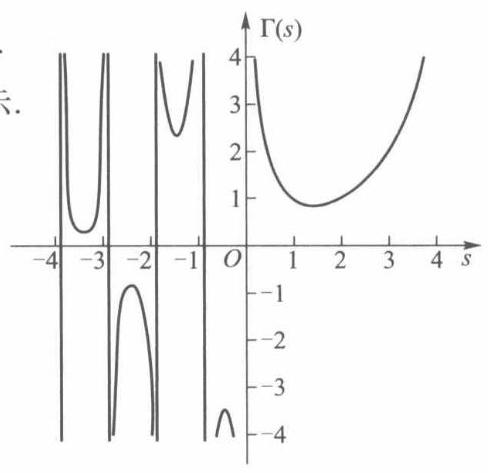
\includegraphics[width=.3\textwidth]{images/P148.jpg}
	\caption{图 $19-2$}
	\label{fig:P148}
\end{figure}

综上所述, \(\Gamma\) 函数的图像如图 19-2 中 \(s > 0\) 部分所示.

4. 延拓 \(\Gamma \left( s\right)\)

改写递推公式(3)为
\[
\Gamma \left( s\right)  = \frac{\Gamma \left( {s + 1}\right) }{s}. \tag{6}
\]
当 \(- 1 < s < 0\) 时,(6) 式右端有意义,于是可应用 (6) 式来定义左端函数 \(\Gamma \left( s\right)\) 在(-1,0)上的值,并且可推得这时 \(\Gamma \left( s\right)  < 0\) .

用同样的方法,利用 \(\Gamma \left( s\right)\) 已在(-1,0)上有定义这一事实,由 (6) 式又可定义 \(\Gamma \left( s\right)\) 在 \(( - 2\) , \(- 1)\) 上的值,而且这时 \(\Gamma \left( s\right)  > 0\) . 依此下去可把 \(\Gamma \left( s\right)\) 延拓到整个数轴 (除了 \(s = 0, - 1\) , －2,…以外),其图像如图 19-2 所示.

5. \(\Gamma \left( s\right)\) 的其他形式

在应用中, \(\Gamma \left( s\right)\) 也常以如下形式出现. 如令 \(x = {y}^{2}\) ,则有
\[
\Gamma \left( s\right)  = {\int }_{0}^{+\infty }{x}^{s - 1}{\mathrm{e}}^{-x}\mathrm{\;d}x = 2{\int }_{0}^{+\infty }{y}^{{2s} - 1}{\mathrm{e}}^{-{y}^{2}}\mathrm{\;d}y\;\left( {s > 0}\right) . \tag{7}
\]
令 \(x = {py}\) ,就有
\[
\Gamma \left( s\right)  = {\int }_{0}^{+\infty }{x}^{s - 1}{\mathrm{e}}^{-x}\mathrm{\;d}x = {p}^{s}{\int }_{0}^{+\infty }{y}^{s - 1}{\mathrm{e}}^{-{py}}\mathrm{\;d}y\;\left( {s > 0,p > 0}\right) . \tag{8}
\]
\subsection{B 函数}

B 函数 (2) 当 \(p < 1\) 时,是以 \(x = 0\) 为瑕点的无界函数反常积分; 当 \(q < 1\) 时,是以 \(x = 1\) 为瑕点的无界函数反常积分. 应用柯西判别法可证得当 \(p > 0,q > 0\) 时这两个无界函数反常积分都收敛,所以函数 \(\mathrm{B}\left( {p,q}\right)\) 的定义域为 \(p > 0,q > 0\) .

虽然 \(\mathrm{B}\left( {p,q}\right)\) 是含两个参量的含参量积分,但与含单参数的含参量积分一样,相应的一致收敛性的定义、判别和性质是完全相同的. 应用这些结论,我们可得以下 \(\mathrm{B}(p\) , \(q)\) 的性质.

1. \(\mathrm{B}\left( {p,q}\right)\) 在定义域 \(p > 0,q > 0\) 内连续

由于对任何 \({p}_{0} > 0,{q}_{0} > 0\) 成立不等式
\[
{x}^{p - 1}{\left( 1 - x\right) }^{q - 1} \leq  {x}^{{p}_{0} - 1}{\left( 1 - x\right) }^{{q}_{0} - 1},p \geq  {p}_{0},q \geq  {q}_{0},
\]
而积分 \({\int }_{0}^{1}{x}^{{p}_{0} - 1}{\left( 1 - x\right) }^{{q}_{0} - 1}\mathrm{\;d}x\) 收敛,故由魏尔斯特拉斯 \(M\) 判别法知 \(\mathrm{B}\left( {p,q}\right)\) 在 \({p}_{0} \leq  p <  + \infty\) , \({q}_{0} \leq  q <  + \infty\) 上一致收敛. 因而推得 \(\mathrm{B}\left( {p,q}\right)\) 在 \(p > 0,q > 0\) 上连续.

2. 对称性: \(\mathrm{B}\left( {p,q}\right)  = \mathrm{B}\left( {q,p}\right)\)

作变换 \(x = 1 - y\) ,得
\[
\mathrm{B}\left( {p,q}\right)  = {\int }_{0}^{1}{x}^{p - 1}{\left( 1 - x\right) }^{q - 1}\mathrm{\;d}x
\]
\[
= {\int }_{0}^{1}{\left( 1 - y\right) }^{p - 1}{y}^{q - 1}\mathrm{\;d}y = \mathrm{B}\left( {q,p}\right) .
\]
3. 递推公式
\[
\mathrm{B}\left( {p,q}\right)  = \frac{q - 1}{p + q - 1}\mathrm{\;B}\left( {p,q - 1}\right) \;\left( {p > 0,q > 1}\right) , \tag{9}
\]
\[
\mathrm{B}\left( {p,q}\right)  = \frac{p - 1}{p + q - 1}\mathrm{\;B}\left( {p - 1,q}\right) \;\left( {p > 1,q > 0}\right) , \tag{10}
\]
\[
\mathrm{B}\left( {p,q}\right)  = \frac{\left( {p - 1}\right) \left( {q - 1}\right) }{\left( {p + q - 1}\right) \left( {p + q - 2}\right) }\mathrm{B}\left( {p - 1,q - 1}\right) \;\left( {p > 1,q > 1}\right) .
\]
%证
\begin{proof}

\end{proof}
下面只证公式 (9) , 公式 (10) 可由对称性及公式 (9) 推得, 而最后一个公式则可由公式 (9), (10) 推得.

当 \(p > 0,q > 1\) 时,有
\[
\mathrm{B}\left( {p,q}\right)  = {\int }_{0}^{1}{x}^{p - 1}{\left( 1 - x\right) }^{q - 1}\mathrm{\;d}x
\]
\[
= {\left. \frac{{x}^{p}{\left( 1 - x\right) }^{q - 1}}{p}\right| }_{0}^{1} + \frac{q - 1}{p}{\int }_{0}^{1}{x}^{p}{\left( 1 - x\right) }^{q - 2}\mathrm{\;d}x
\]
\[
= \frac{q - 1}{p}{\int }_{0}^{1}\left\lbrack  {{x}^{p - 1} - {x}^{p - 1}\left( {1 - x}\right) }\right\rbrack  {\left( 1 - x\right) }^{q - 2}\mathrm{\;d}x
\]
\[
= \frac{q - 1}{p}{\int }_{0}^{1}{x}^{p - 1}{\left( 1 - x\right) }^{q - 2}\mathrm{\;d}x - \frac{q - 1}{p}{\int }_{0}^{1}{x}^{p - 1}{\left( 1 - x\right) }^{q - 1}\mathrm{\;d}x
\]
\[
= \frac{q - 1}{p}\mathrm{\;B}\left( {p,q - 1}\right)  - \frac{q - 1}{p}\mathrm{\;B}\left( {p,q}\right) ,
\]
移项并整理就得 (9).

4. \(\mathrm{B}\left( {p,q}\right)\) 的其他形式

在应用中 \(\mathrm{B}\) 函数也常以如下形式出现. 如令 \(x = {\cos }^{2}\varphi\) ,则有
\[
\mathrm{B}\left( {p,q}\right)  = 2{\int }_{0}^{\frac{\pi }{2}}{\sin }^{{2q} - 1}\varphi {\cos }^{{2p} - 1}\varphi \mathrm{d}\varphi . \tag{11}
\]
令 \(x = \frac{y}{1 + y},1 - x = \frac{1}{1 + y},\mathrm{\;d}x = \frac{\mathrm{d}y}{{\left( 1 + y\right) }^{2}}\) ,则有
\[
\mathrm{B}\left( {p,q}\right)  = {\int }_{0}^{+\infty }\frac{{y}^{p - 1}}{{\left( 1 + y\right) }^{p + q}}\mathrm{\;d}y.
\]
考察 \({\int }_{1}^{+\infty }\frac{{y}^{p - 1}}{{\left( 1 + y\right) }^{p + q}}\mathrm{\;d}y\) . 令 \(y = \frac{1}{t}\) ,则有
\[
{\int }_{1}^{+\infty }\frac{{y}^{p - 1}}{{\left( 1 + y\right) }^{p + q}}\mathrm{\;d}y =  - {\int }_{1}^{0}\frac{{t}^{q - 1}}{{\left( 1 + t\right) }^{p + q}}\mathrm{\;d}t.
\]
所以
\[
\mathrm{B}\left( {p,q}\right)  = {\int }_{0}^{1}\frac{{y}^{p - 1} + {y}^{q - 1}}{{\left( 1 + y\right) }^{p + q}}\mathrm{\;d}y.
\]
\subsection{ \(\Gamma\) 函数与 \(\mathrm{B}\) 函数之间的关系}

当 \(m,n\) 为正整数时,反复应用 \(\mathrm{B}\) 函数的递推公式可得
\[
\mathrm{B}\left( {m,n}\right)  = \frac{n - 1}{m + n - 1}\mathrm{\;B}\left( {m,n - 1}\right)
\]
\[
= \frac{n - 1}{m + n - 1}\frac{n - 2}{m + n - 2}\cdots \frac{1}{m + 1}\mathrm{\;B}\left( {m,1}\right) .
\]
又由于 \(\mathrm{B}\left( {m,1}\right)  = {\int }_{0}^{1}{x}^{m - 1}\mathrm{\;d}x = \frac{1}{m}\) ,所以
\[
\mathrm{B}\left( {m,n}\right)  = \frac{n - 1}{m + n - 1}\frac{n - 2}{m + n - 2}\cdots \frac{1}{m + 1}\frac{1}{m} \cdot  \frac{\left( {m - 1}\right) !}{\left( {m - 1}\right) !}
\]
\[
= \frac{\left( {n - 1}\right) !\left( {m - 1}\right) !}{\left( {m + n - 1}\right) !},
\]
即
\[
\mathrm{B}\left( {m,n}\right)  = \frac{\Gamma \left( n\right) \Gamma \left( m\right) }{\Gamma \left( {n + m}\right) }. \tag{12}
\]
对于任何正实数 \(p,q\) 也有相同的关系:
\[
\mathrm{B}\left( {p,q}\right)  = \frac{\Gamma \left( p\right) \Gamma \left( q\right) }{\Gamma \left( {p + q}\right) }\;\left( {p > 0,q > 0}\right) . \tag{13}
\]
这个关系式我们将在第二十一章 §8 中加以证明.

\subsection{习题 19.3}

1. 计算 \(\Gamma \left( \frac{5}{2}\right) ,\Gamma \left( {-\frac{5}{2}}\right) ,\Gamma \left( {\frac{1}{2} + n}\right) ,\Gamma \left( {\frac{1}{2} - n}\right)\) .

2. 计算 \({\int }_{0}^{\frac{\pi }{2}}{\sin }^{2n}u\mathrm{\;d}u,{\int }_{0}^{\frac{\pi }{2}}{\sin }^{{2n} + 1}u\mathrm{\;d}u\) .

3. 证明下列各式:

(1) \(\Gamma \left( a\right)  = {\int }_{0}^{1}{\left( \ln \frac{1}{x}\right) }^{a - 1}\mathrm{\;d}x,a > 0\) ;

(2) \({\int }_{0}^{+\infty }\frac{{x}^{a - 1}}{1 + x}\mathrm{\;d}x = \Gamma \left( a\right) \Gamma \left( {1 - a}\right) ,0 < a < 1\) ；

(3) \({\int }_{0}^{1}{x}^{p - 1}{\left( 1 - {x}^{r}\right) }^{q - 1}\mathrm{\;d}x = \frac{1}{r}\mathrm{\;B}\left( {\frac{p}{r},q}\right) ,p > 0,q > 0,r > 0\) ;

(4) \({\int }_{0}^{+\infty }\frac{\mathrm{d}x}{1 + {x}^{4}} = \frac{\pi }{2\sqrt{2}}\) .

4. 证明公式
\[
\mathrm{B}\left( {p,q}\right)  = \mathrm{B}\left( {p + 1,q}\right)  + \mathrm{B}\left( {p,q + 1}\right) .
\]
5. 已知 \(\Gamma \left( \frac{1}{2}\right)  = \sqrt{\pi }\) ,试证
\[
{\int }_{-\infty }^{+\infty }{x}^{2}{\mathrm{e}}^{-{x}^{2}}\mathrm{\;d}x = \frac{\sqrt{\pi }}{2}.
\]
6. 试将下列积分用欧拉积分表示, 并指出参量的取值范围:

(1) \({\int }_{0}^{\frac{\pi }{2}}{\sin }^{m}x{\cos }^{n}x\mathrm{\;d}x\) ;

(2) \({\int }_{0}^{1}{\left( \ln \frac{1}{x}\right) }^{p}\mathrm{\;d}x\) .

\section{总练习题}

1. 在区间 \(1 \leq  x \leq  3\) 上用线性函数 \(a + {bx}\) 近似代替 \(f\left( x\right)  = {x}^{2}\) ,试求 \(a,b\) ,使得积分 \({\int }_{1}^{3}{\left( a + bx - {x}^{2}\right) }^{2}\mathrm{\;d}x\) 取最小值.

2. 设 \(u\left( x\right)  = {\int }_{0}^{1}k\left( {x,y}\right) v\left( y\right) \mathrm{d}y\) ,其中
\[
k\left( {x,y}\right)  = \left\{  \begin{array}{l} x\left( {1 - y}\right) ,x \leq  y, \\  y\left( {1 - x}\right) ,x > y, \end{array}\right.
\]
\(v\left( y\right)\) 为 \(\left\lbrack  {0,1}\right\rbrack\) 上的连续函数,证明
\[
{u}^{\prime \prime }\left( x\right)  =  - v\left( x\right) .
\]


3. 求函数
\[
F\left( a\right)  = {\int }_{0}^{+\infty }\frac{\sin \left( {1 - {a}^{2}}\right) x}{x}\mathrm{\;d}x
\]
的不连续点,并作函数 \(F\left( a\right)\) 的图像.

4. 证明: 若 \({\int }_{0}^{+\infty }f\left( {x,t}\right) \mathrm{d}t\) 在 \(x \in  \left( {0, + \infty }\right)\) 上一致收敛于 \(F\left( x\right)\) ,且 \(\mathop{\lim }\limits_{{x \rightarrow   + \infty }}f\left( {x,t}\right)  = \varphi \left( t\right)\) 对任意 \(t \in  \left\lbrack  {a,b}\right\rbrack   \subset  \left( {0, + \infty }\right)\) 一致地成立 (即对任意 \(\varepsilon  > 0\) ,存在 \(M > 0\) ,当 \(x > M\) 时, \(\left| {f\left( {x,t}\right)  - \varphi \left( t\right) }\right|  < \varepsilon\) 对一切 \(t \in\)  \(\left\lbrack  {a,b}\right\rbrack\) 成立),则有
\[
\mathop{\lim }\limits_{{x \rightarrow   + \infty }}F\left( x\right)  = {\int }_{0}^{+\infty }\varphi \left( t\right) \mathrm{d}t.
\]
5. 设 \(f\left( x\right)\) 为二阶可微函数, \(F\left( x\right)\) 为可微函数. 证明函数
\[
u\left( {x,t}\right)  = \frac{1}{2}\left\lbrack  {f\left( {x - {at}}\right)  + f\left( {x + {at}}\right) }\right\rbrack   + \frac{1}{2a}{\int }_{x - {at}}^{x + {at}}F\left( z\right) \mathrm{d}z
\]
满足弦振动方程
\[
\frac{{\partial }^{2}u}{\partial {t}^{2}} = {a}^{2}\frac{{\partial }^{2}u}{\partial {x}^{2}}
\]
及初值条件 \(u\left( {x,0}\right)  = f\left( x\right) ,{u}_{t}\left( {x,0}\right)  = F\left( x\right)\) .

6. 证明:

(1) \({\int }_{0}^{1}\frac{\ln x}{1 - x}\mathrm{\;d}x =  - \frac{{\pi }^{2}}{6}\) ;

(2) \({\int }_{0}^{u}\frac{\ln \left( {1 - t}\right) }{t}\mathrm{\;d}t =  - \mathop{\sum }\limits_{{n = 1}}^{\infty }\frac{{u}^{n}}{{n}^{2}},0 \leq  u \leq  1\) .

